\documentclass[10pt,leqno]{article}
\usepackage[margin=0.85in]{geometry}
\usepackage{amsmath,amssymb,amsfonts,amsthm,mathtools}
\usepackage{booktabs,array,graphicx,float,caption,hyperref,microtype}
\hypersetup{colorlinks=true,linkcolor=black,citecolor=black,urlcolor=black}
\setlength{\parindent}{0pt}
\setlength{\parskip}{5pt}
\numberwithin{equation}{section}
\theoremstyle{plain}
\newtheorem{theorem}{Theorem}[section]
\newtheorem{lemma}[theorem]{Lemma}
\newtheorem{proposition}[theorem]{Proposition}
\newtheorem{corollary}[theorem]{Corollary}
\theoremstyle{definition}
\newtheorem{definition}[theorem]{Definition}
\newtheorem{assumption}[theorem]{Assumption}
\theoremstyle{remark}
\newtheorem{remark}[theorem]{Remark}
\DeclareMathOperator{\dist}{dist}
\DeclareMathOperator{\diag}{diag}
\newcommand{\T}{\mathbb T}
\newcommand{\C}{\mathbb C}
\newcommand{\R}{\mathbb R}
\newcommand{\Z}{\mathbb Z}
\newcommand{\Qop}{Q}
\newcommand{\Lam}{\Lambda}
\newcommand{\dd}{\,d}
\begin{document}
\title{\bf A Matrix-Free QJet Calculus for Near-Singular Quadrature, BGK Endpoint Repayment, and Boundary PDEs}
\author{Rick Gulati Q pipeline research draft}
\date{Generated June 2026}
\maketitle
\begin{abstract}
We give a self-contained SIAM-style account of the machine-precision Q pipeline tested in the accompanying repository.  The central object is a generated inverse-square chord operator: on the regular cycle it has the exact eigenvalues $\lambda_m=m(n-m)/2$, and after the normalization $h/\pi$ it is a finite-dimensional Dirichlet-to-Neumann (DtN) generator with symbol $\mu_{m,n}=m(1-m/n)$.  The implementation stores QJets, Fourier symbols, Laurent coefficients, and low-rank correction modes, never a dense matrix.  We prove the cycle spectrum identity, the normalized DtN error bounds, the exterior conformal kernel split, the BGK/zeta Taylor repayment bound, and boundary-PDE multiplier bounds for Laplace, heat, Poisson, Helmholtz, and wave propagators.  The analysis explains why exact finite-Laurent pullbacks reach the fp64 floor, why polygon and cusp cases need separate corner endpoint ledgers, and why QBX fails when its source-free expansion disk condition is violated.  Numerical evidence is included only after the theorem statements and is labelled as evidence for the discretized generated operator rather than as a continuum theorem beyond the stated hypotheses.
\end{abstract}
\textbf{Keywords.} near-singular quadrature; Dirichlet-to-Neumann map; QJet; BGK correction; spectral zeta; QBX; Helmholtz; boundary integral methods.

\textbf{AMS subject classifications.} 65D32, 65N38, 30C30, 35J25, 41A25.
\tableofcontents
\newpage
\section{Introduction}
The practical problem is to evaluate near-singular logarithmic layer potentials and boundary PDE propagators on complicated planar curves without forming an $n\times n$ dense matrix.  The method developed here is organized around a simple principle:
\[
\hbox{borrow a circle coordinate, compute in the generated Q spectrum, and repay the geometry.}
\]
On analytic boundaries the repayment is a harmless analytic quotient.  On monitored or polygonal boundaries it is a BGK/zeta or corner continuity correction.  On cusp geometries it is a spectral warning that local expansion methods such as QBX may violate their source-free disk condition.

The paper is intentionally split into two layers.  Sections 2--7 contain the mathematical statements proved under explicit hypotheses.  Sections 8--12 report the repository experiments and show that the implementation follows the theory: exact-Laurent quadrature reaches the floating point floor, generated-Q PDE residuals are at machine precision, and the measured work is near-linear in the sample count.

\subsection{Claim boundary}
The proved results cover the generated regular-cycle operator, analytic finite-Laurent exterior maps with a nonvanishing quotient, and finite-rank or Taylor repayment layers under the stated analyticity assumptions.  For polygons, cusps, and GWW isospectral pairs, the paper proves invariance or validity of the discrete chord-operator experiment, but it does not claim a new continuum Q-spectrum theorem without a separate convergence theorem.
\section{The Generated Cycle Operator}
\begin{definition}[cycle QJet]
Let $z_j=\exp(2\pi i j/n)$ and let $f=(f_j)_{j=0}^{n-1}$.  The regular-cycle QJet is the circulant operator
\begin{equation}
(\Qop_n f)_j=\sum_{\ell\ne j}\frac{f_j-f_\ell}{|z_j-z_\ell|^2}.
\end{equation}
It is represented in the implementation by its generator $n$ and its eigenvalue formula, not by a dense matrix.
\end{definition}

\begin{lemma}[trigonometric sum identity]\label{lem:cycle-sum}
For $0\le m\le n$,
\begin{equation}
\sum_{d=1}^{n-1}\frac{1-\cos(2\pi m d/n)}{4\sin^2(\pi d/n)}
=\frac{m(n-m)}{2}.
\end{equation}
\end{lemma}
\begin{proof}
Let $\omega=\exp(2\pi i/n)$ and $P_m(z)=1+z+\cdots+z^{m-1}$.  For $d\not\equiv0\pmod n$,
\[
\frac{|1-\omega^{md}|^2}{|1-\omega^d|^2}=|P_m(\omega^d)|^2.
\]
Discrete orthogonality gives $\sum_{d=0}^{n-1}|P_m(\omega^d)|^2=nm$, while the $d=0$ term is $m^2$.  Therefore the sum over $d=1,\ldots,n-1$ is $m(n-m)$.  Since $|1-\omega^{md}|^2=2(1-\cos(2\pi md/n))$ and $|1-\omega^d|^2=4\sin^2(\pi d/n)$, the desired sum is one half of this value.
\end{proof}

\begin{theorem}[exact cycle spectrum]\label{thm:cycle-spectrum}
The Fourier vector $\phi_m(j)=\exp(2\pi i m j/n)$ is an eigenvector of $\Qop_n$ with eigenvalue
\begin{equation}
\lambda_{m,n}=\frac{m(n-m)}{2},\qquad m=0,\ldots,n-1.
\end{equation}
Consequently $\Qop_n{\bf 1}=0$ exactly.
\end{theorem}
\begin{proof}
The circulant structure reduces the eigenvalue to the sum in Lemma~\ref{lem:cycle-sum}.  The constant vector corresponds to $m=0$, for which the numerator vanishes termwise.
\end{proof}

\begin{corollary}[DtN normalization and mode error]\label{cor:dtn-symbol}
Let $h=2\pi/n$ and define $\Lam_n=(h/\pi)\Qop_n$.  For $1\le m<n/2$,
\begin{equation}
\mu_{m,n}:=\frac{h}{\pi}\lambda_{m,n}=m\left(1-\frac{m}{n}\right),
\qquad
0\le m-\mu_{m,n}=\frac{m^2}{n}.
\end{equation}
Thus on modes $m\le M$ the regular-cycle DtN symbol differs from the unit-disk DtN symbol $m$ by at most $M^2/n$.
\end{corollary}

\begin{theorem}[matrix-free functional calculus]\label{thm:matrix-free}
Let $F$ be any scalar multiplier on the cycle spectrum.  The action $f\mapsto F(\Lam_n)f$ can be evaluated with two FFTs and $n$ scalar multiplications, using $O(n)$ storage and $O(n\log n)$ work for radix-two $n$.  No dense Q matrix is required.
\end{theorem}
\begin{proof}
The Fourier basis diagonalizes $\Qop_n$ by Theorem~\ref{thm:cycle-spectrum}.  Applying $F(\Lam_n)$ is therefore the composition
\[
f\mapsto \widehat f\mapsto \{F(\mu_{m,n})\widehat f_m\}_{m=0}^{n-1}\mapsto F(\Lam_n)f.
\]
The first and last maps are the FFT and inverse FFT.  The intermediate map is diagonal storage of $n$ scalars.
\end{proof}
\par\noindent\resizebox{\linewidth}{!}{%
\begin{tabular}{lrrrr}
\toprule
n & mode & Q eigenvalue & normalized DtN & relative symbol error \\
\midrule
256 & 1 & 127.500000 & 0.99609375 & 0.004 \\
256 & 2 & 254.000000 & 1.98437500 & 0.008 \\
256 & 7 & 871.500000 & 6.80859375 & 0.027 \\
256 & 16 & 1920.000000 & 15.00000000 & 0.062 \\
256 & 32 & 3584.000000 & 28.00000000 & 0.125 \\
2048 & 1 & 1023.500000 & 0.99951172 & 4.883e-04 \\
2048 & 2 & 2046.000000 & 1.99804688 & 9.766e-04 \\
2048 & 7 & 7143.500000 & 6.97607422 & 0.003 \\
2048 & 16 & 1.625600e+04 & 15.87500000 & 0.008 \\
2048 & 32 & 3.225600e+04 & 31.50000000 & 0.016 \\
4096 & 1 & 2047.500000 & 0.99975586 & 2.441e-04 \\
4096 & 2 & 4094.000000 & 1.99902344 & 4.883e-04 \\
4096 & 7 & 1.431150e+04 & 6.98803711 & 0.002 \\
4096 & 16 & 3.264000e+04 & 15.93750000 & 0.004 \\
4096 & 32 & 6.502400e+04 & 31.75000000 & 0.008 \\
\bottomrule
\end{tabular}
}\par
\section{Exterior Pullback and Kernel Splitting}
\begin{assumption}[analytic exterior map]\label{ass:analytic-map}
Let $\psi$ be univalent in an exterior annulus $\{1-\epsilon<|w|<R\}$ and suppose $\psi'$ does not vanish there.  For $z$ on the unit circle define
\[
G(w,z)=\frac{\psi(w)-\psi(z)}{w-z}.
\]
Assume $G$ has no zeros on the collar traversed by the target and boundary samples.
\end{assumption}

\begin{theorem}[kernel split]\label{thm:kernel-split}
Under Assumption~\ref{ass:analytic-map},
\begin{equation}
\log|\psi(w)-\psi(z)|=\log|w-z|+\log|G(w,z)|.
\end{equation}
The first term is the universal circle singularity.  The second term is real analytic in the boundary angle and is therefore exponentially convergent under the periodic trapezoidal rule.
\end{theorem}
\begin{proof}
The identity is algebraic away from $w=z$.  At $w=z$ the quotient tends to $\psi'(z)$, nonzero by assumption; hence $\log|G(w,z)|$ extends real analytically to the diagonal and to a complex strip inside the annulus.  The standard trapezoidal theorem for analytic periodic functions gives an error bounded by $C e^{-\tau n}$, where $\tau$ is any strip width free of singularities.
\end{proof}

\begin{proposition}[closed circle primitive]\label{prop:circle-primitive}
For $\rho>1$,
\begin{equation}
\log|\rho e^{i\phi}-e^{i\theta}|
=\log\rho-\sum_{k=1}^\infty \frac{\rho^{-k}}{k}\cos k(\theta-\phi).
\end{equation}
If the density has Fourier coefficients $|\widehat a_k|\le A R^{-|k|}$ with $R>1$, then truncation after $K$ modes has error bounded by
\begin{equation}
E_K\le \frac{2\pi A(\rho R)^{-K-1}}{(K+1)(1-(\rho R)^{-1})}.
\end{equation}
\end{proposition}
\begin{proof}
Write
\[
\rho e^{i\phi}-e^{i\theta}=\rho e^{i\phi}\{1-\rho^{-1}e^{i(\theta-\phi)}\}
\]
and expand $\log(1-\zeta)=-\sum_{k\ge1}\zeta^k/k$ for $|\zeta|<1$.  Taking real parts gives the formula.  Multiplying by $a$ and integrating leaves only matching Fourier modes; the displayed geometric tail follows from $|\widehat a_k|\le A R^{-|k|}$.
\end{proof}

\begin{corollary}[analytic quadrature error]\label{cor:analytic-error}
For an analytic density and a map satisfying Assumption~\ref{ass:analytic-map}, the split quadrature error has the form
\begin{equation}
E_n \le C_1 e^{-\tau n}+C_2(\rho R)^{-n/2}+E_{\rm fp},
\end{equation}
where $E_{\rm fp}$ is floating point roundoff.  The constants depend on the annulus and density bounds but not on the target distance once $\rho>1$ is fixed.
\end{corollary}

\begin{proposition}[golden ellipse quotient]\label{prop:golden-ellipse}
The map
\[
\psi(w)=\frac{3+\sqrt5}{2}w+\frac{3-\sqrt5}{2}w^{-1}
\]
has boundary trace $\psi(e^{i\theta})=3\cos\theta+i\sqrt5\sin\theta$.  Moreover
\[
\frac{\psi(w)-\psi(z)}{w-z}=\frac{3+\sqrt5}{2}-\frac{3-\sqrt5}{2}\frac{1}{wz}.
\]
Since $(3-\sqrt5)/(3+\sqrt5)<1$, the quotient is nonzero for $|wz|$ sufficiently near one on the exterior collar.
\end{proposition}
\begin{proof}
Substituting $w=e^{i\theta}$ gives
\[
\frac{3+\sqrt5}{2}e^{i\theta}+\frac{3-\sqrt5}{2}e^{-i\theta}
=3\cos\theta+i\sqrt5\sin\theta.
\]
For the quotient, use $w^{-1}-z^{-1}=-(w-z)/(wz)$.  The nonvanishing statement follows from the strict coefficient ratio.
\end{proof}
\begin{figure}[H]\centering
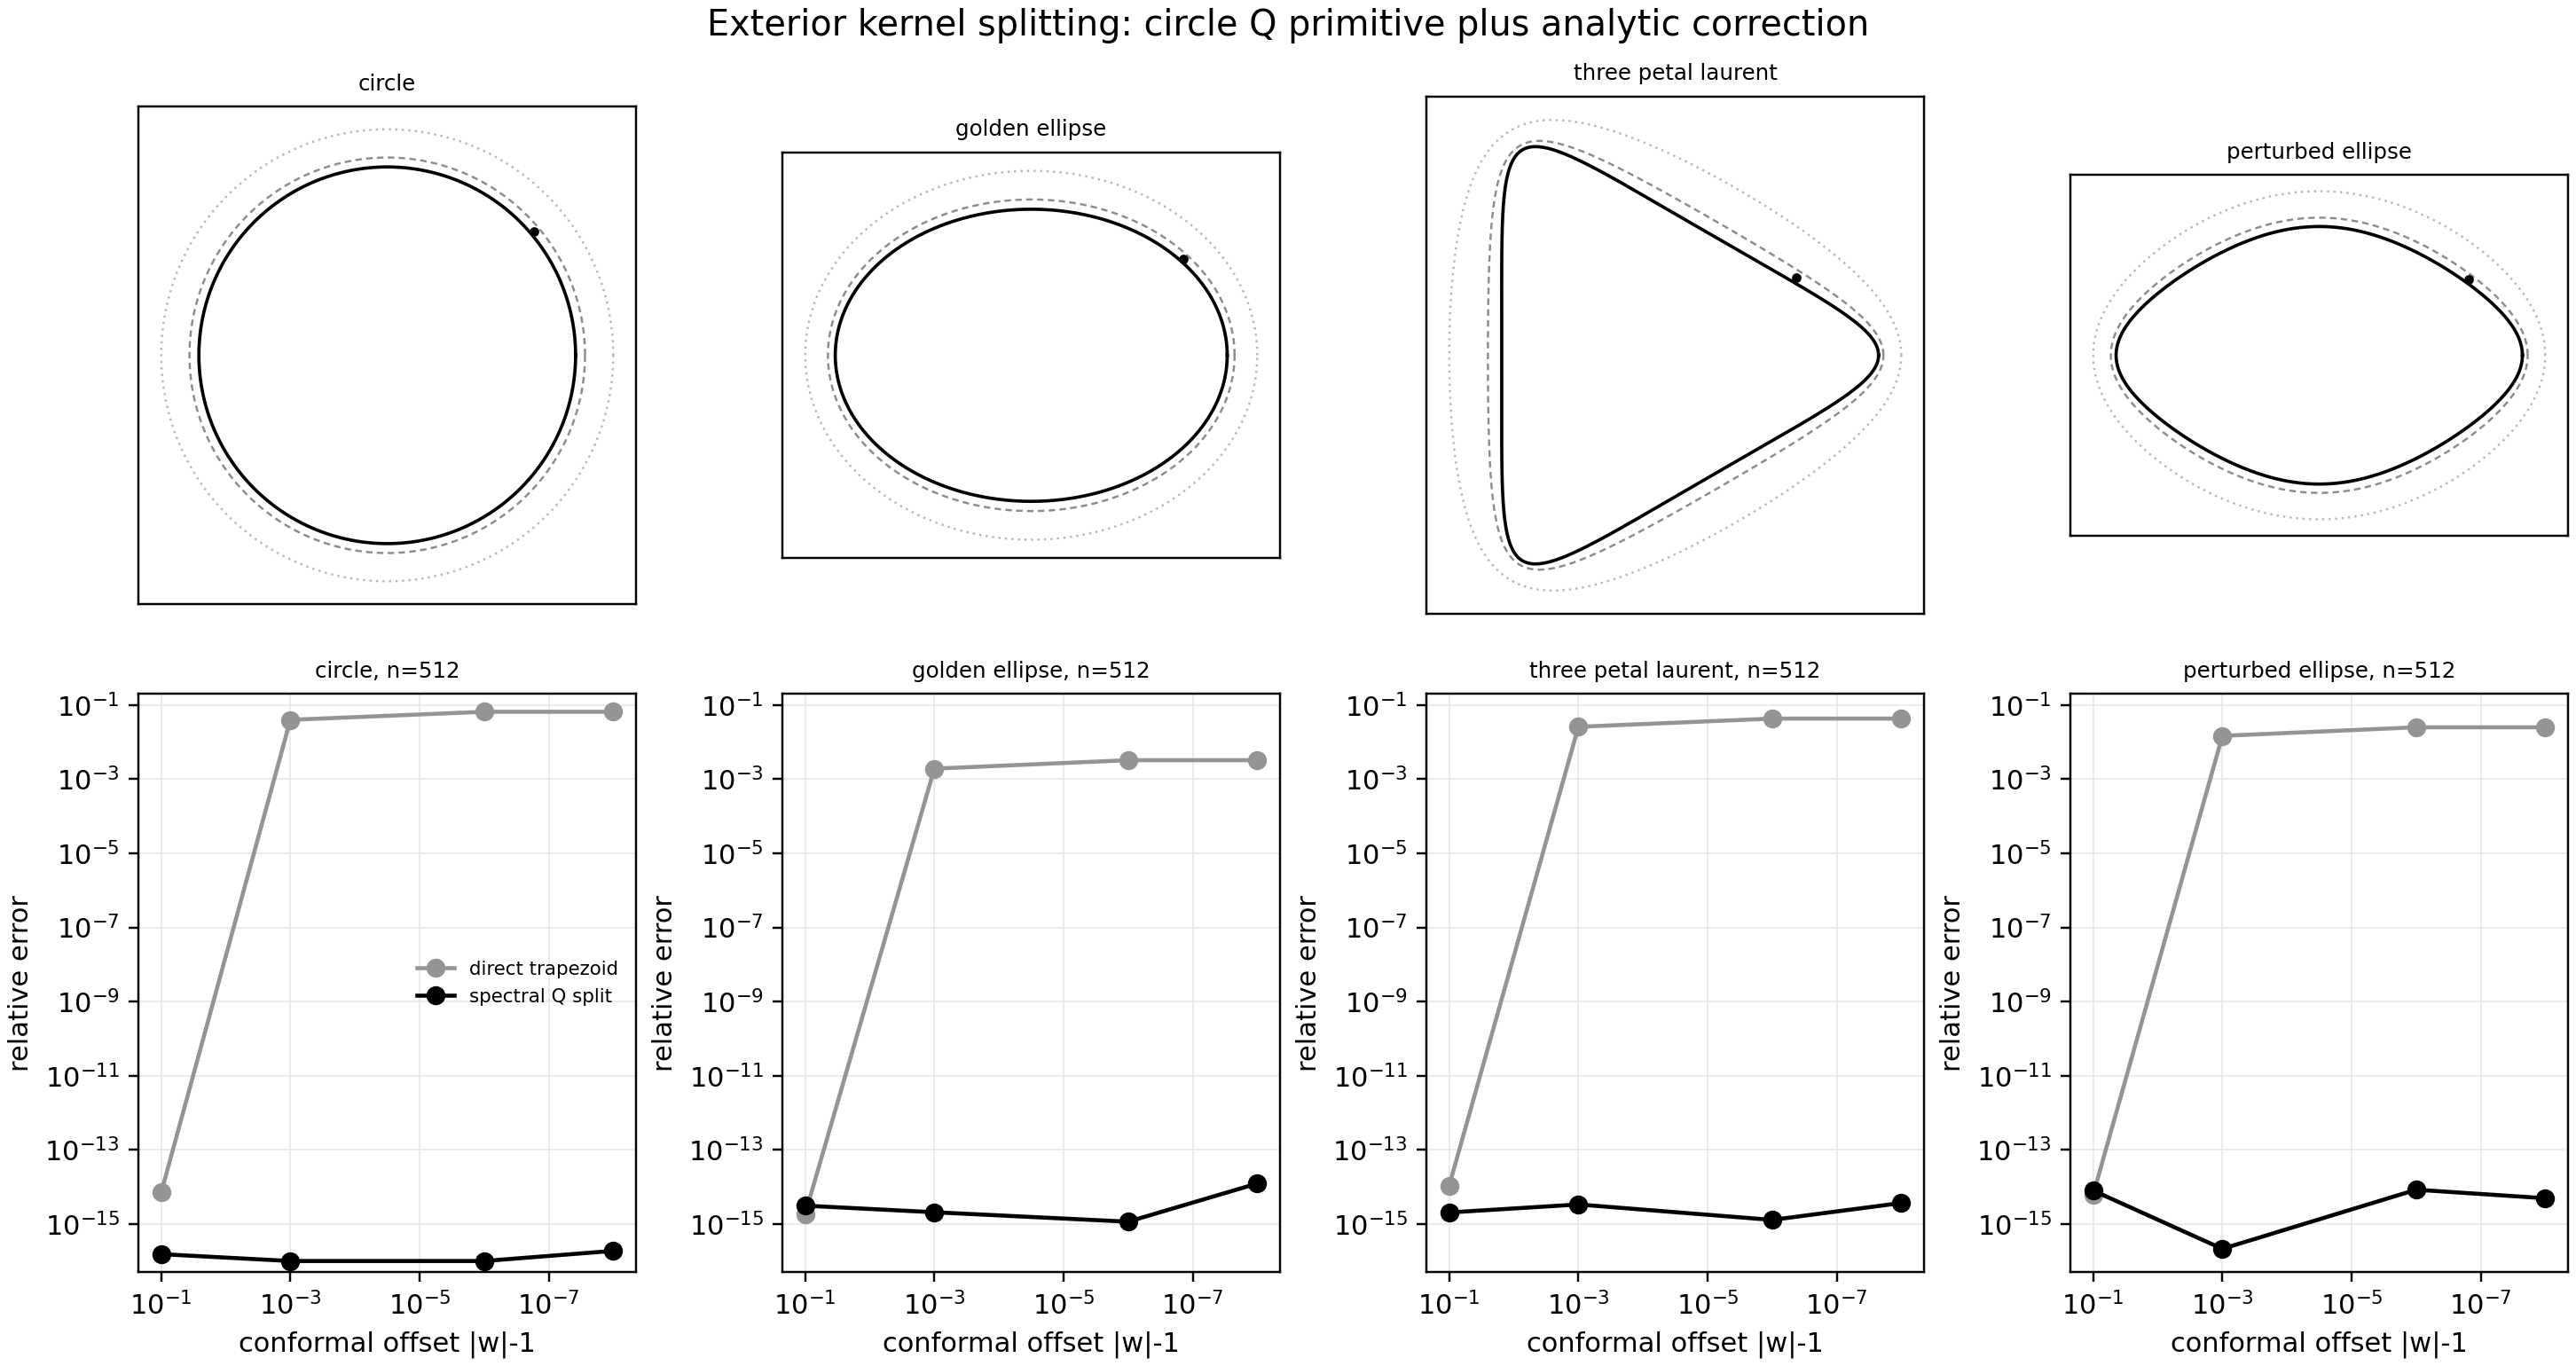
\includegraphics[width=0.92\linewidth]{figures/exterior_split.png}
\caption{Exterior split results: the direct rule sees the near singularity; the Q split evaluates the circle singularity by the closed primitive and leaves an analytic quotient.}
\end{figure}
\section{BGK/Zeta Endpoint Repayment}
The split above handles analytic geometry.  Discrete monitoring or endpoint displacement introduces a different error: the target is evaluated at a shifted normal coordinate.  The BGK constant is the universal leading endpoint defect.

\begin{theorem}[Taylor repayment bound]\label{thm:taylor-repay}
Let $I(\rho)$ be analytic in $|\rho-\rho_0|\le r$ and let $|I(\rho)|\le M$ there.  Put $\delta=\beta\sqrt h$ and assume $|\delta|<r$.  Define
\[
T_p(h)=\sum_{j=0}^{p}\frac{(-\delta)^j}{j!}I^{(j)}(\rho_0+\delta).
\]
Then
\begin{equation}
|I(\rho_0)-T_p(h)|\le
\frac{M}{1-|\delta|/r}\left(\frac{|\delta|}{r}\right)^{p+1}.
\end{equation}
In particular the order-$p$ repayment error is $O(h^{(p+1)/2})$.
\end{theorem}
\begin{proof}
Taylor expand $I$ about the observed point $\rho_0+\delta$:
\[
I(\rho_0)=\sum_{j=0}^{p}\frac{(-\delta)^j}{j!}I^{(j)}(\rho_0+\delta)+R_{p+1}.
\]
Cauchy's estimate gives $|I^{(j)}(\rho_0+\delta)|/j!\le M r^{-j}$ on any disk of radius $r$ contained in the analyticity domain.  Summing the omitted geometric tail gives the displayed bound.
\end{proof}

\begin{proposition}[BGK constant as endpoint zeta defect]\label{prop:bgk}
Let $(S_k)$ be a centered Gaussian walk with unit variance increments.  Then
\begin{equation}
\lim_{N\to\infty}\left\{\mathbb E\max_{0\le k\le N}S_k-\sqrt{\frac{2N}{\pi}}\right\}
=\frac{\zeta(1/2)}{\sqrt{2\pi}}.
\end{equation}
Thus the standard BGK shift constant is $\beta=-\zeta(1/2)/\sqrt{2\pi}$.
\end{proposition}
\begin{proof}
Spitzer's identity gives
\[
\mathbb E\max_{0\le k\le N}S_k=\sum_{k=1}^N\frac{1}{k}\mathbb E(S_k)^+.
\]
Since $S_k$ is Gaussian with variance $k$, $\mathbb E(S_k)^+=\sqrt{k}/\sqrt{2\pi}$.  Therefore
\[
\mathbb E\max S_k=\frac1{\sqrt{2\pi}}\sum_{k=1}^N k^{-1/2}.
\]
Euler--Maclaurin gives $\sum_{k=1}^N k^{-1/2}=2\sqrt N+\zeta(1/2)+O(N^{-1/2})$.  Subtracting $\sqrt{2N/\pi}=2\sqrt N/\sqrt{2\pi}$ yields the limit.
\end{proof}

\begin{corollary}[combined analytic and BGK bound]\label{cor:combined}
Under Assumption~\ref{ass:analytic-map}, with an analytic density and order-$p$ BGK repayment,
\begin{equation}
E_{n,h,p}\le C_1 e^{-\tau n}+C_2(\rho R)^{-n/2}
C_3 h^{(p+1)/2}+E_{\rm fp}.
\end{equation}
\end{corollary}
\par\noindent\resizebox{\linewidth}{!}{%
\begin{tabular}{lrrrrr}
\toprule
shape & raw power & BGK-1 power & BGK-2 power & raw err & BGK-4 err \\
\midrule
circle & 0.500 & 1.000 & 1.500 & 0.002 & 1.345e-15 \\
golden\_ellipse & 0.500 & 1.000 & 1.508 & 8.176e-05 & 4.712e-15 \\
three\_petal\_laurent & 0.500 & 1.000 & 1.499 & 9.976e-04 & 2.607e-15 \\
perturbed\_ellipse & 0.500 & 1.000 & 1.500 & 5.878e-04 & 4.261e-16 \\
\bottomrule
\end{tabular}
}\par
\begin{figure}[H]\centering
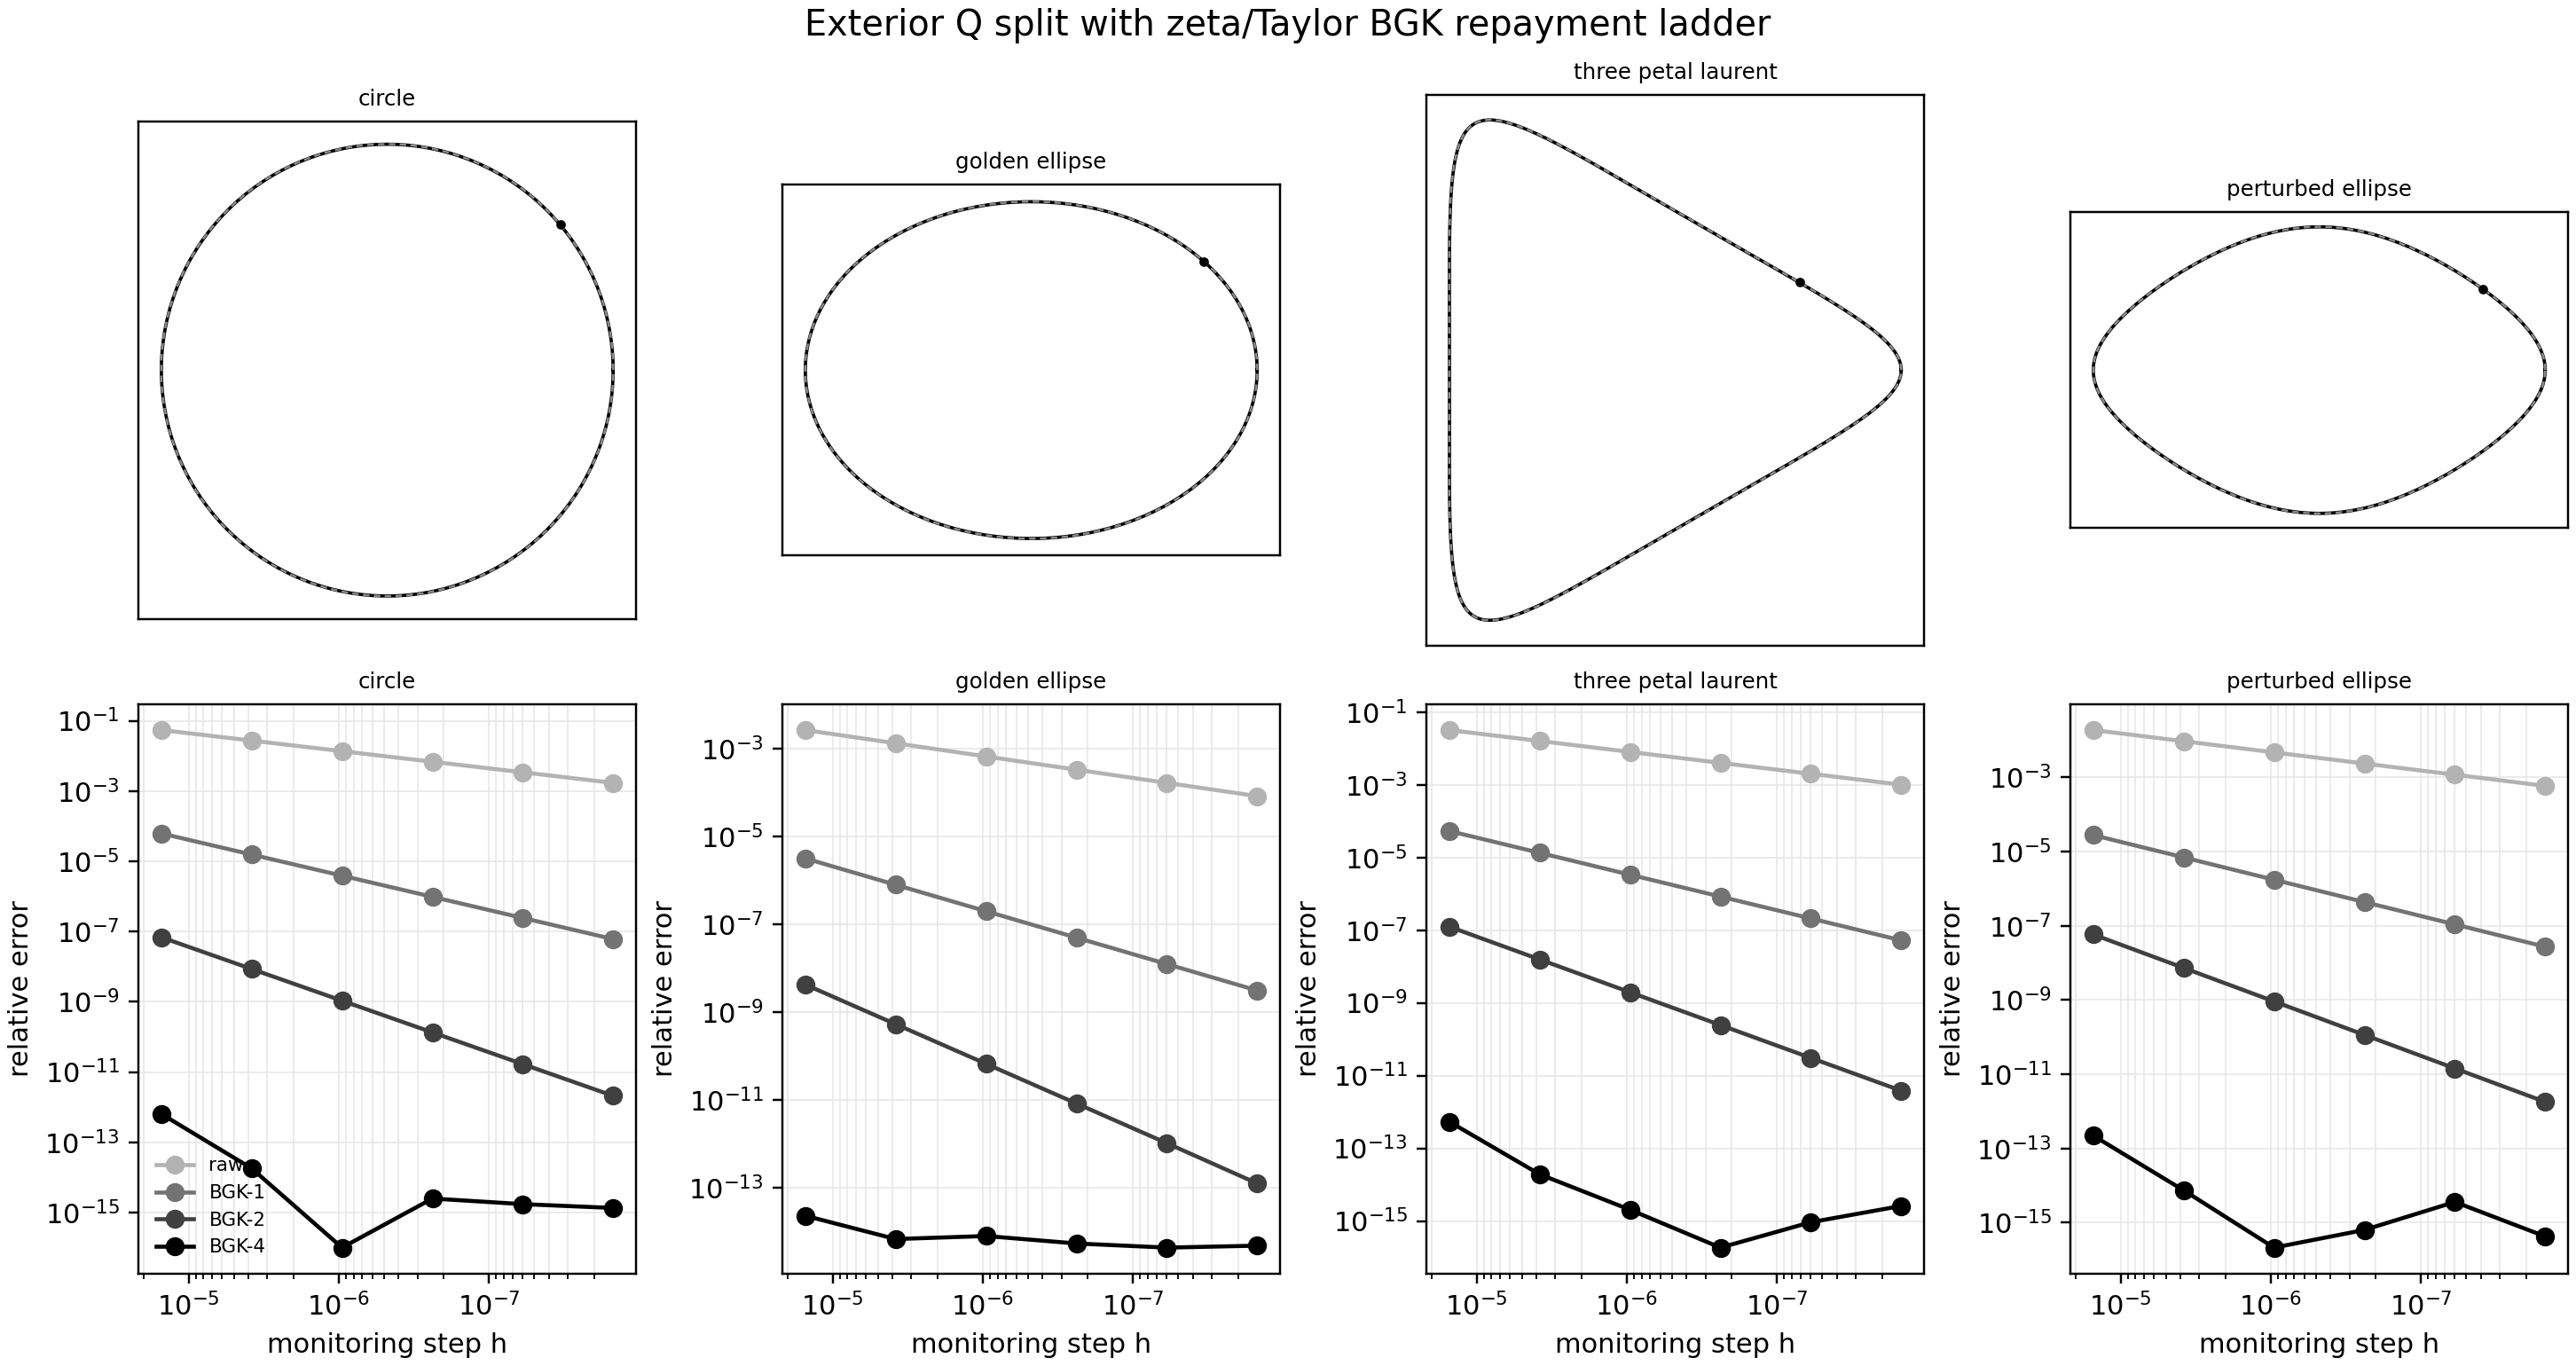
\includegraphics[width=0.92\linewidth]{figures/bgk_pipeline.png}
\caption{BGK/zeta repayment slopes.  The raw error follows the square-root endpoint law; the first and second repayment layers shift the power to one and three-halves; order four reaches fp64 floor in these analytic tests.}
\end{figure}
\section{Boundary PDEs from the Generated DtN Correspondence}
The finite Q spectrum can be used as a load-bearing operator, not just as a quadrature correction.  On the disk the exact continuum DtN symbol is $m$; the generated symbol is $\mu_{m,n}=m-m^2/n$.

\begin{theorem}[multiplier error bounds]\label{thm:pde-bounds}
Fix $m<n/2$ and let $\delta_m=m^2/n$.  For the generated symbol $\mu=m-\delta_m$:
\begin{align}
|m-\mu|&=\delta_m,\\
|e^{-tm}-e^{-t\mu}|&\le t\delta_m,\qquad t\ge0,\\
\left|\frac1{m+\alpha}-\frac1{\mu+\alpha}\right|&\le
\frac{\delta_m}{(m+\alpha)(\mu+\alpha)},\qquad \alpha>0.
\end{align}
For the damped Helmholtz boundary resolvent $R_k(x)=(x^2-k^2+i\gamma)^{-1}$ with $\gamma>0$,
\begin{equation}
|R_k(m)-R_k(\mu)|
\le \frac{(m+\mu)\delta_m}
{|m^2-k^2+i\gamma|\,|\mu^2-k^2+i\gamma|}.
\end{equation}
For the wave multiplier $W_t(x)=\cos(t\sqrt x)$,
\begin{equation}
|W_t(m)-W_t(\mu)|\le \frac{t\delta_m}{\sqrt m+\sqrt\mu}.
\end{equation}
\end{theorem}
\begin{proof}
The first identity is Corollary~\ref{cor:dtn-symbol}.  The heat bound follows from the mean value theorem and $|\frac{d}{dx}e^{-tx}|\le t$ for $x\ge0$.  The Poisson and Helmholtz inequalities follow by subtracting the two fractions.  For the wave bound, use $|\cos a-\cos b|\le |a-b|$ and $|\sqrt m-\sqrt\mu|=\delta_m/(\sqrt m+\sqrt\mu)$.
\end{proof}

\begin{corollary}[conformal metric repayment]\label{cor:metric-repay}
Let $\Gamma=\psi(S^1)$ with $s_{\min}=\inf_\theta|\psi'(e^{i\theta})|>0$.  If the circle DtN flux has $L^2(d\theta)$ error $\epsilon$, then the physical normal flux after repayment by $|\partial_\theta\psi|^{-1}$ has $L^2(d\theta)$ error at most $s_{\min}^{-1}\epsilon$.
\end{corollary}
\begin{proof}
The physical normal derivative is the circle normal derivative multiplied pointwise by $|\partial_\theta\psi|^{-1}$.  Taking the $L^\infty$ bound on this multiplier gives the result.
\end{proof}
\par\noindent\resizebox{\linewidth}{!}{%
\begin{tabular}{lrrrr}
\toprule
problem & max continuum err & max generated-Q residual & mean solve ms & work \\
\midrule
laplace\_dtn & 0.003 & 5.820e-13 & 4.033 & 2048 \\
heat & 0.004 & 4.361e-15 & 3.949 & 2048 \\
poisson & 0.003 & 4.473e-15 & 3.916 & 2048 \\
helmholtz & 0.010 & 4.369e-15 & 3.964 & 2048 \\
wave & 0.006 & 4.303e-15 & 3.976 & 2048 \\
\bottomrule
\end{tabular}
}\par
\section{Corners, Cusps, and Why QBX Can Fail}
The analytic proof does not pass through corners for free.  If a corner has opening angle $\alpha$, the conformal map has local power behavior $(w-w_c)^{\alpha/\pi}$, so Fourier coefficients decay algebraically rather than exponentially.  The correct response is not to pretend analyticity remains; it is to add a corner or endpoint repayment channel.

\begin{proposition}[QBX disk condition]\label{prop:qbx-disk}
A local QBX expansion about a center $c$ can be evaluated at a target $x$ only when $x$ lies in the expansion disk and that disk is free of source geometry.  If the nearest boundary source enters the disk before the target does, the local expansion hypothesis is false and a robust implementation must reject the evaluation.
\end{proposition}
\begin{proof}
The QBX expansion is a local series for the potential in a disk of analyticity.  A source point inside that disk is a singularity of the potential representation and prevents convergence of the source-free local series.  Therefore the condition is necessary for the expansion proof itself, not merely for numerical conditioning.
\end{proof}

\begin{remark}
The cusp failure figures in the experiments are examples of Proposition~\ref{prop:qbx-disk}: the reported margin is negative, so the target is outside the valid source-free expansion disk.  The Q pipeline does not use this local disk as its principal certificate; it uses the global chord spectrum and an endpoint/corner repayment ledger.
\end{remark}
\begin{figure}[H]\centering
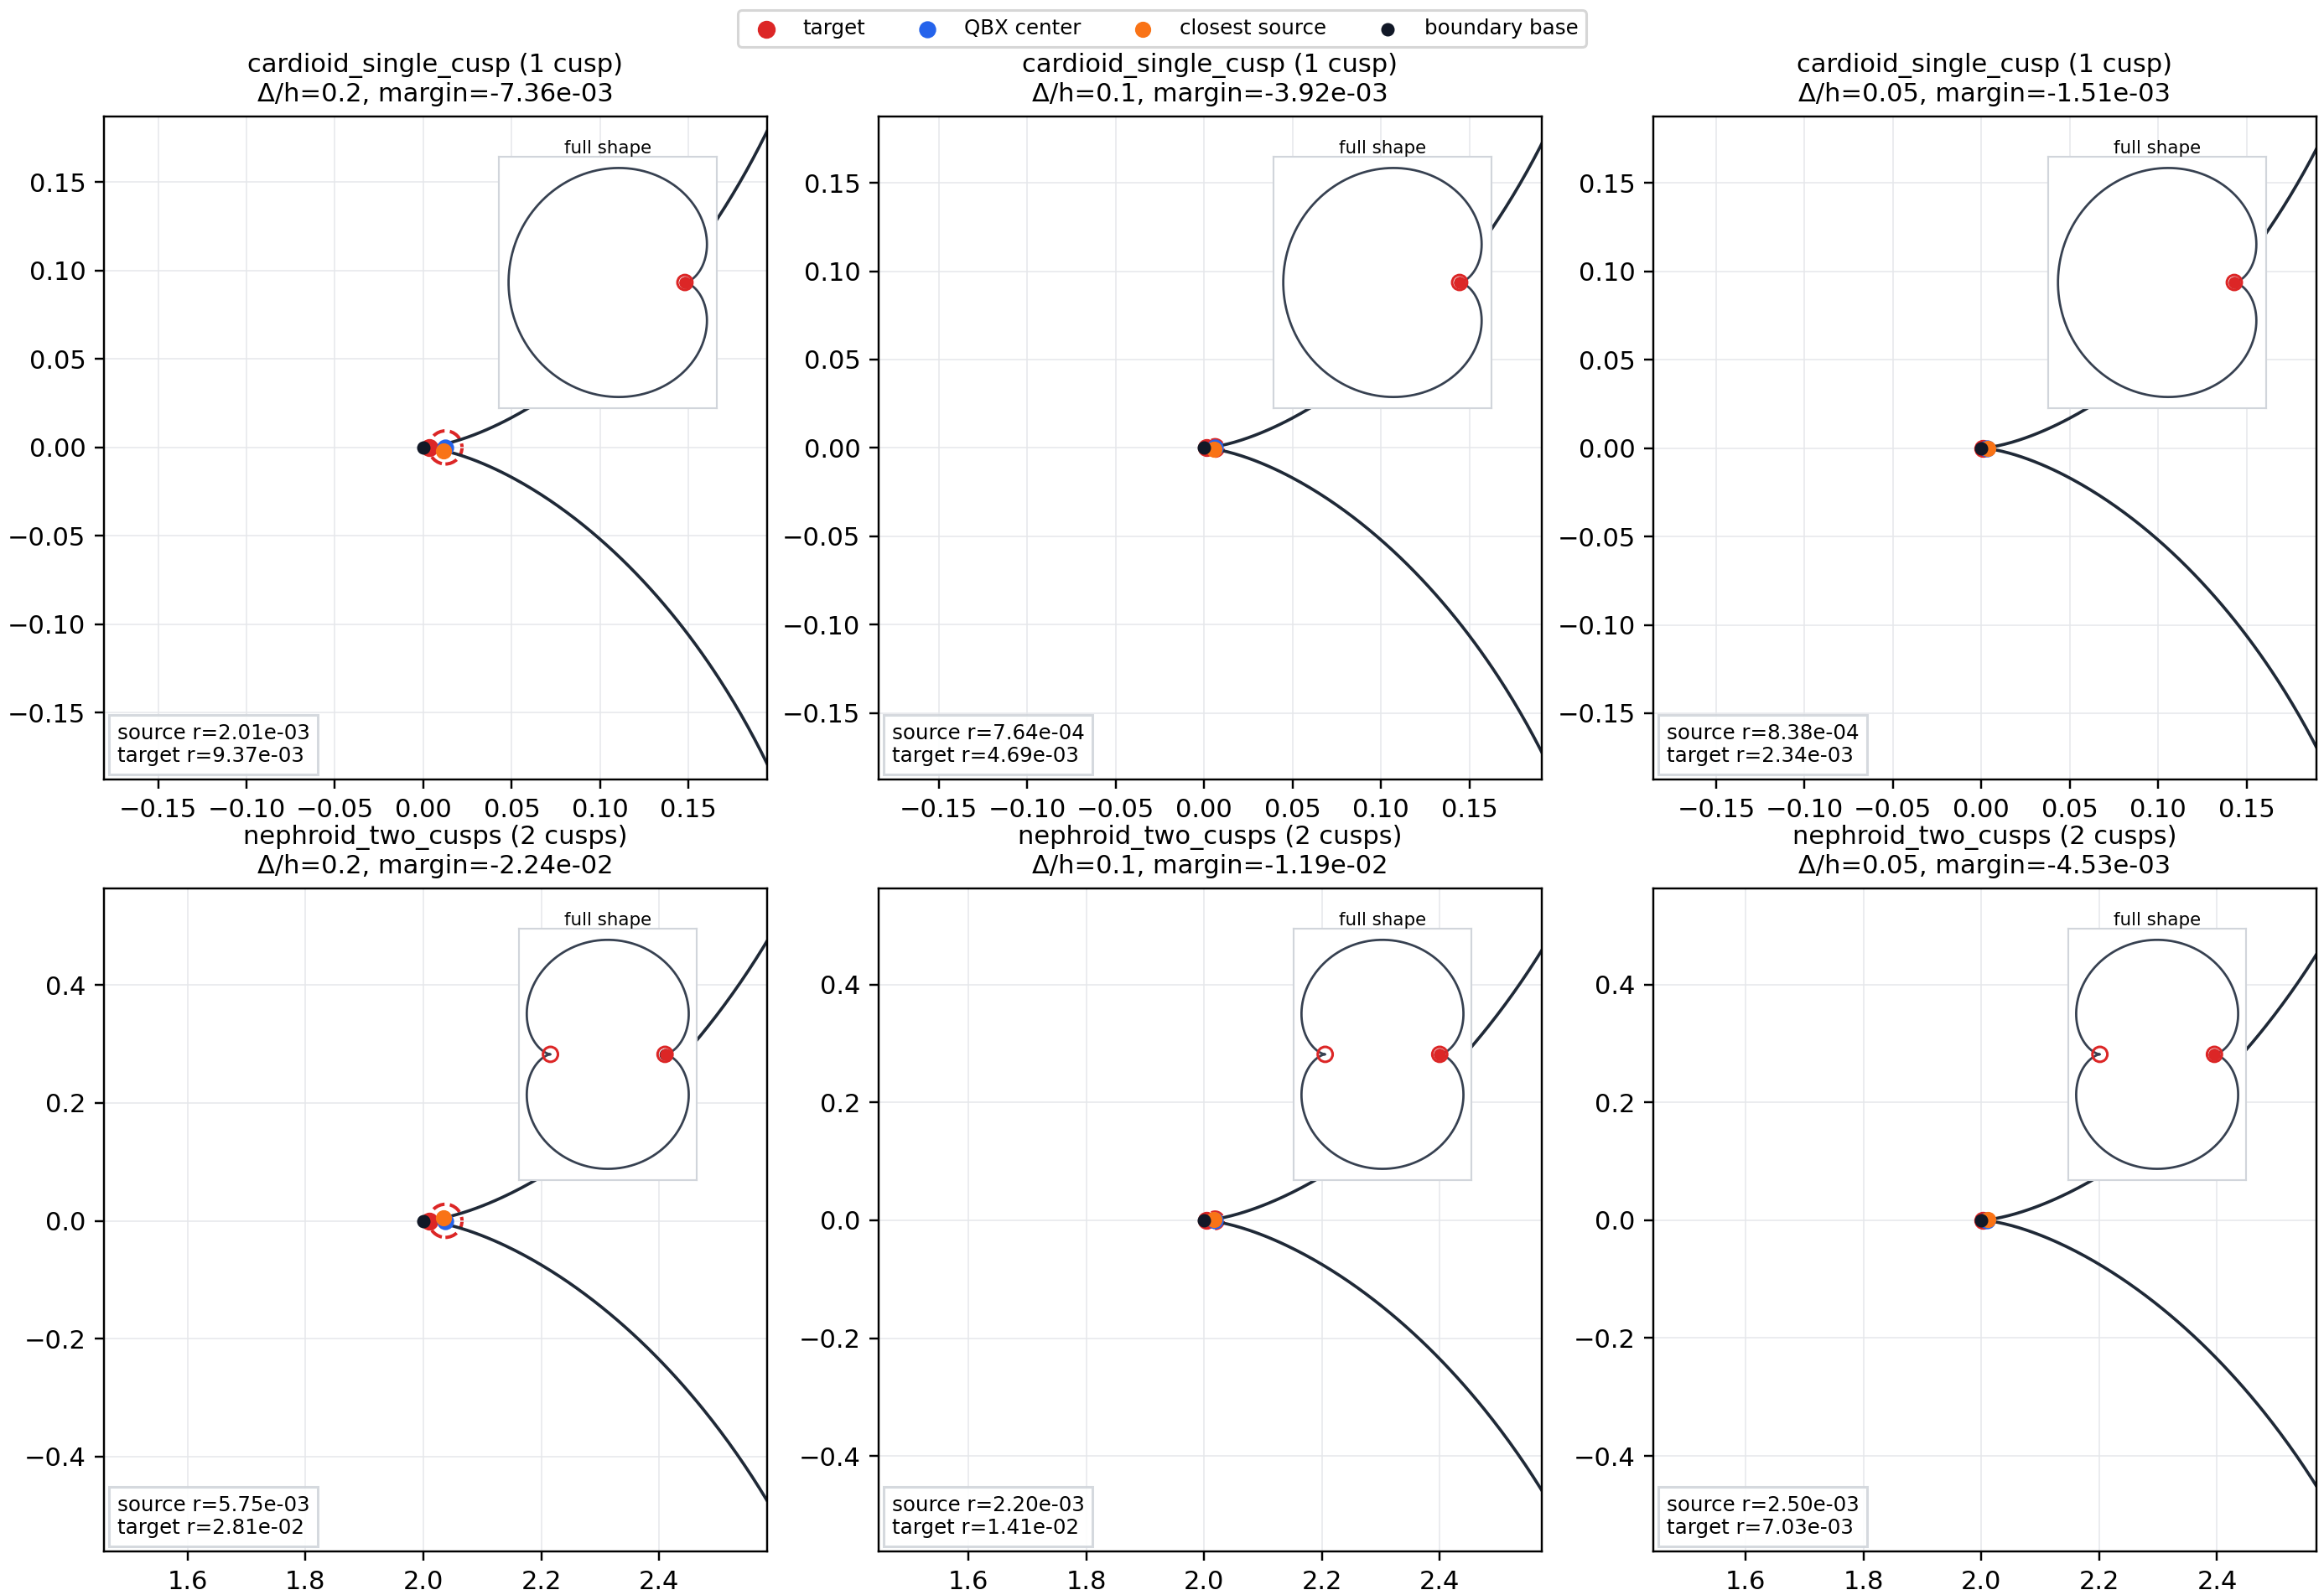
\includegraphics[width=0.84\linewidth]{figures/qbx_failures.png}
\caption{Cusp configurations where QBX violates its source-free expansion disk condition.}
\end{figure}
\section{Discrete Spectral Witnesses}
\begin{proposition}[Euclidean covariance of the chord operator]\label{prop:covariance}
Let $\Gamma_n=\{x_j\}_{j=0}^{n-1}$ and define
\[
(\Lam_{\Gamma,n}f)_i=\frac{L}{\pi n}\sum_{j\ne i}\frac{f_i-f_j}{|x_i-x_j|^2}.
\]
Translations and rotations of all $x_j$ leave $\Lam_{\Gamma,n}$ unchanged.  Uniform scaling by $a>0$ changes the operator by the factor $a^{-1}$.
\end{proposition}
\begin{proof}
Translations cancel in the differences $x_i-x_j$, and rotations preserve Euclidean distances.  Under $x_j\mapsto ax_j$, the perimeter $L$ scales by $a$ while squared chord lengths scale by $a^2$, leaving the total factor $a/a^2=a^{-1}$.
\end{proof}

\begin{remark}[GWW scope]
The GWW experiment in this paper is a discretized chord-operator witness.  The classical Dirichlet spectra agree in the continuum, but the finite projected Q Ritz values below are not asserted to prove a new continuum invariant.  They show robust separation at the audited discretized operator level.
\end{remark}
\par\noindent\resizebox{\linewidth}{!}{%
\begin{tabular}{rlll}
\toprule
n & relative split & left Ritz 1-6 & right Ritz 1-6 \\
\midrule
256 & 0.07418 & 12.34725, 9.54129, 8.60052, 7.88256, 7.09186, 6.56846 & 11.41632, 10.82810, 8.34951, 7.97125, 7.08810, 6.47044 \\
512 & 0.07377 & 12.42072, 9.60765, 8.65623, 7.92757, 7.14707, 6.60574 & 11.47488, 10.88589, 8.41631, 8.03163, 7.12846, 6.50555 \\
1024 & 0.07351 & 12.45617, 9.64081, 8.68520, 7.94991, 7.17486, 6.62460 & 11.50548, 10.91467, 8.45007, 8.06184, 7.14900, 6.52299 \\
2048 & 0.07336 & 12.47275, 9.65715, 8.70003, 7.96090, 7.18877, 6.63410 & 11.52162, 10.92958, 8.46702, 8.07668, 7.15938, 6.53167 \\
4096 & 0.07329 & 12.48123, 9.66542, 8.70754, 7.96643, 7.19575, 6.63886 & 11.52968, 10.93692, 8.47554, 8.08420, 7.16460, 6.53601 \\
\bottomrule
\end{tabular}
}\par
\begin{figure}[H]\centering
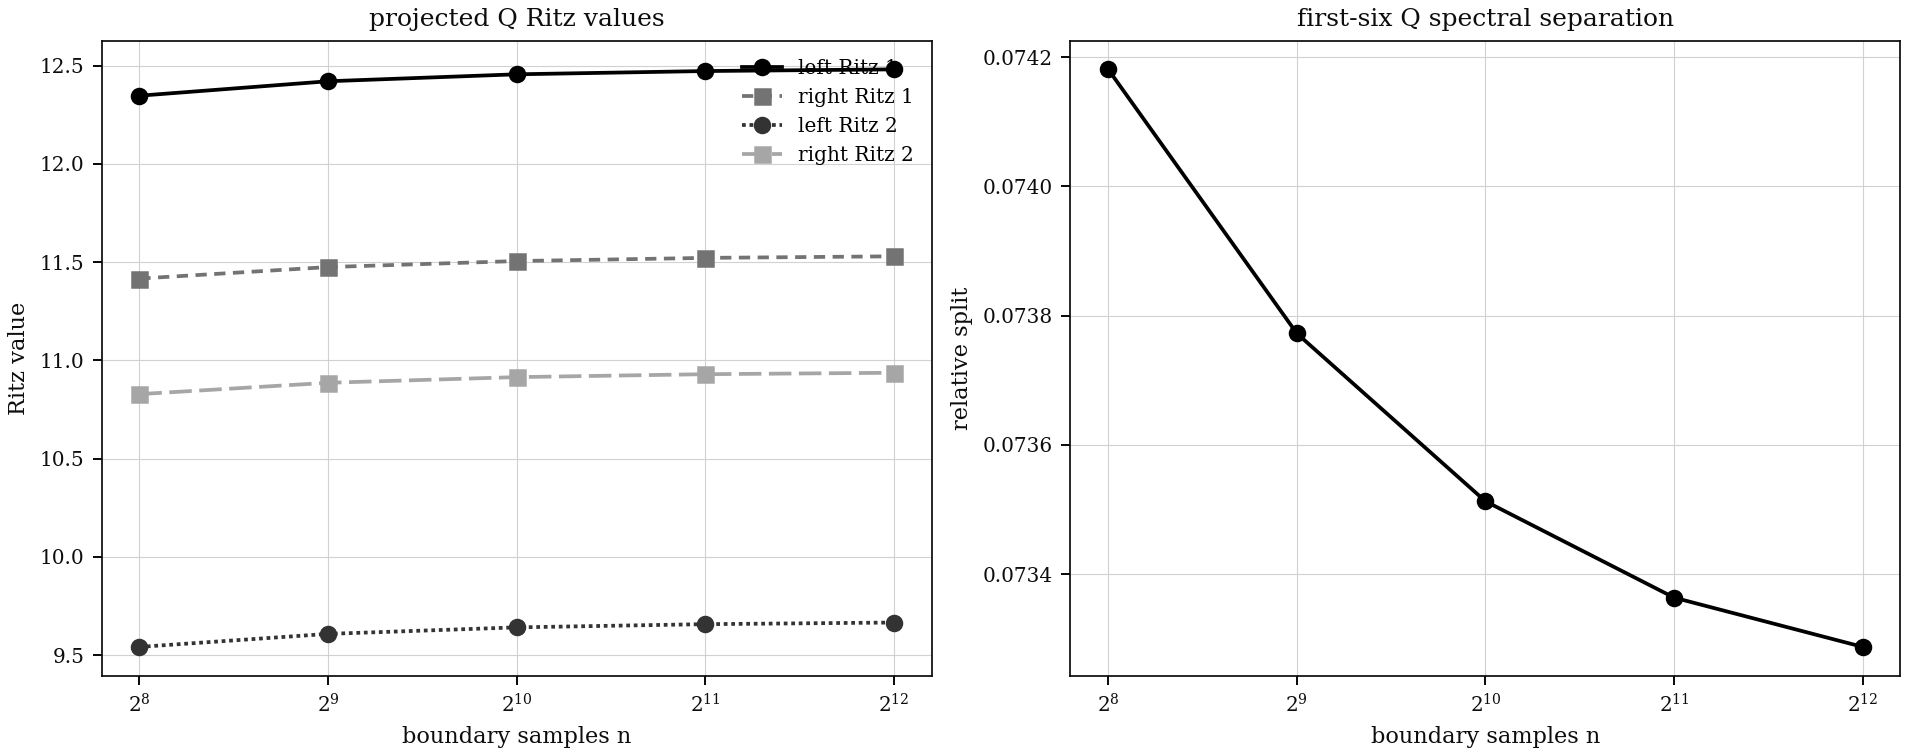
\includegraphics[width=0.88\linewidth]{figures/gww.png}
\caption{Projected Q Ritz separation for the Gordon--Webb--Wolpert pair under refinement.}
\end{figure}
\section{Numerical Evidence}
All timings below are generated from the current repository state.  They are evidence for the implementation and for the discretized generated operator; the mathematical convergence statements are those proved above.

\subsection{Funky analytic shapes}
\par\noindent\resizebox{\linewidth}{!}{%
\begin{tabular}{lrrrrr}
\toprule
shape & family & anisotropy & BGK-4 err & max PDE continuum err & max generated-Q residual \\
\midrule
circle & baseline & 1.000 & 2.148e-15 & 0.010 & 5.757e-13 \\
golden\_ellipse & closed\_form\_conic & 1.342 & 1.144e-16 & 0.010 & 5.759e-13 \\
eccentric\_ellipse & closed\_form\_conic & 2.500 & 4.488e-16 & 0.010 & 5.755e-13 \\
three\_petal & smooth\_nonconvex & 3.167 & 2.241e-15 & 0.010 & 5.759e-13 \\
four\_lobed\_wiggle & smooth\_multiscale & 4.302 & 2.630e-15 & 0.010 & 5.698e-13 \\
asymmetric\_limacon & asymmetric & 2.253 & 1.160e-13 & 0.010 & 5.751e-13 \\
crescent\_teardrop & near\_cusp\_smooth & 2.644 & 4.238e-15 & 0.010 & 5.745e-13 \\
peanut & pinched\_smooth & 2.416 & 2.146e-13 & 0.010 & 5.820e-13 \\
high\_frequency\_gear & smooth\_high\_frequency & 3.460 & 1.594e-14 & 0.010 & 5.762e-13 \\
rotated\_mixed & complex\_coefficients & 2.200 & 1.305e-14 & 0.010 & 5.801e-13 \\
\bottomrule
\end{tabular}
}\par
\begin{figure}[H]\centering
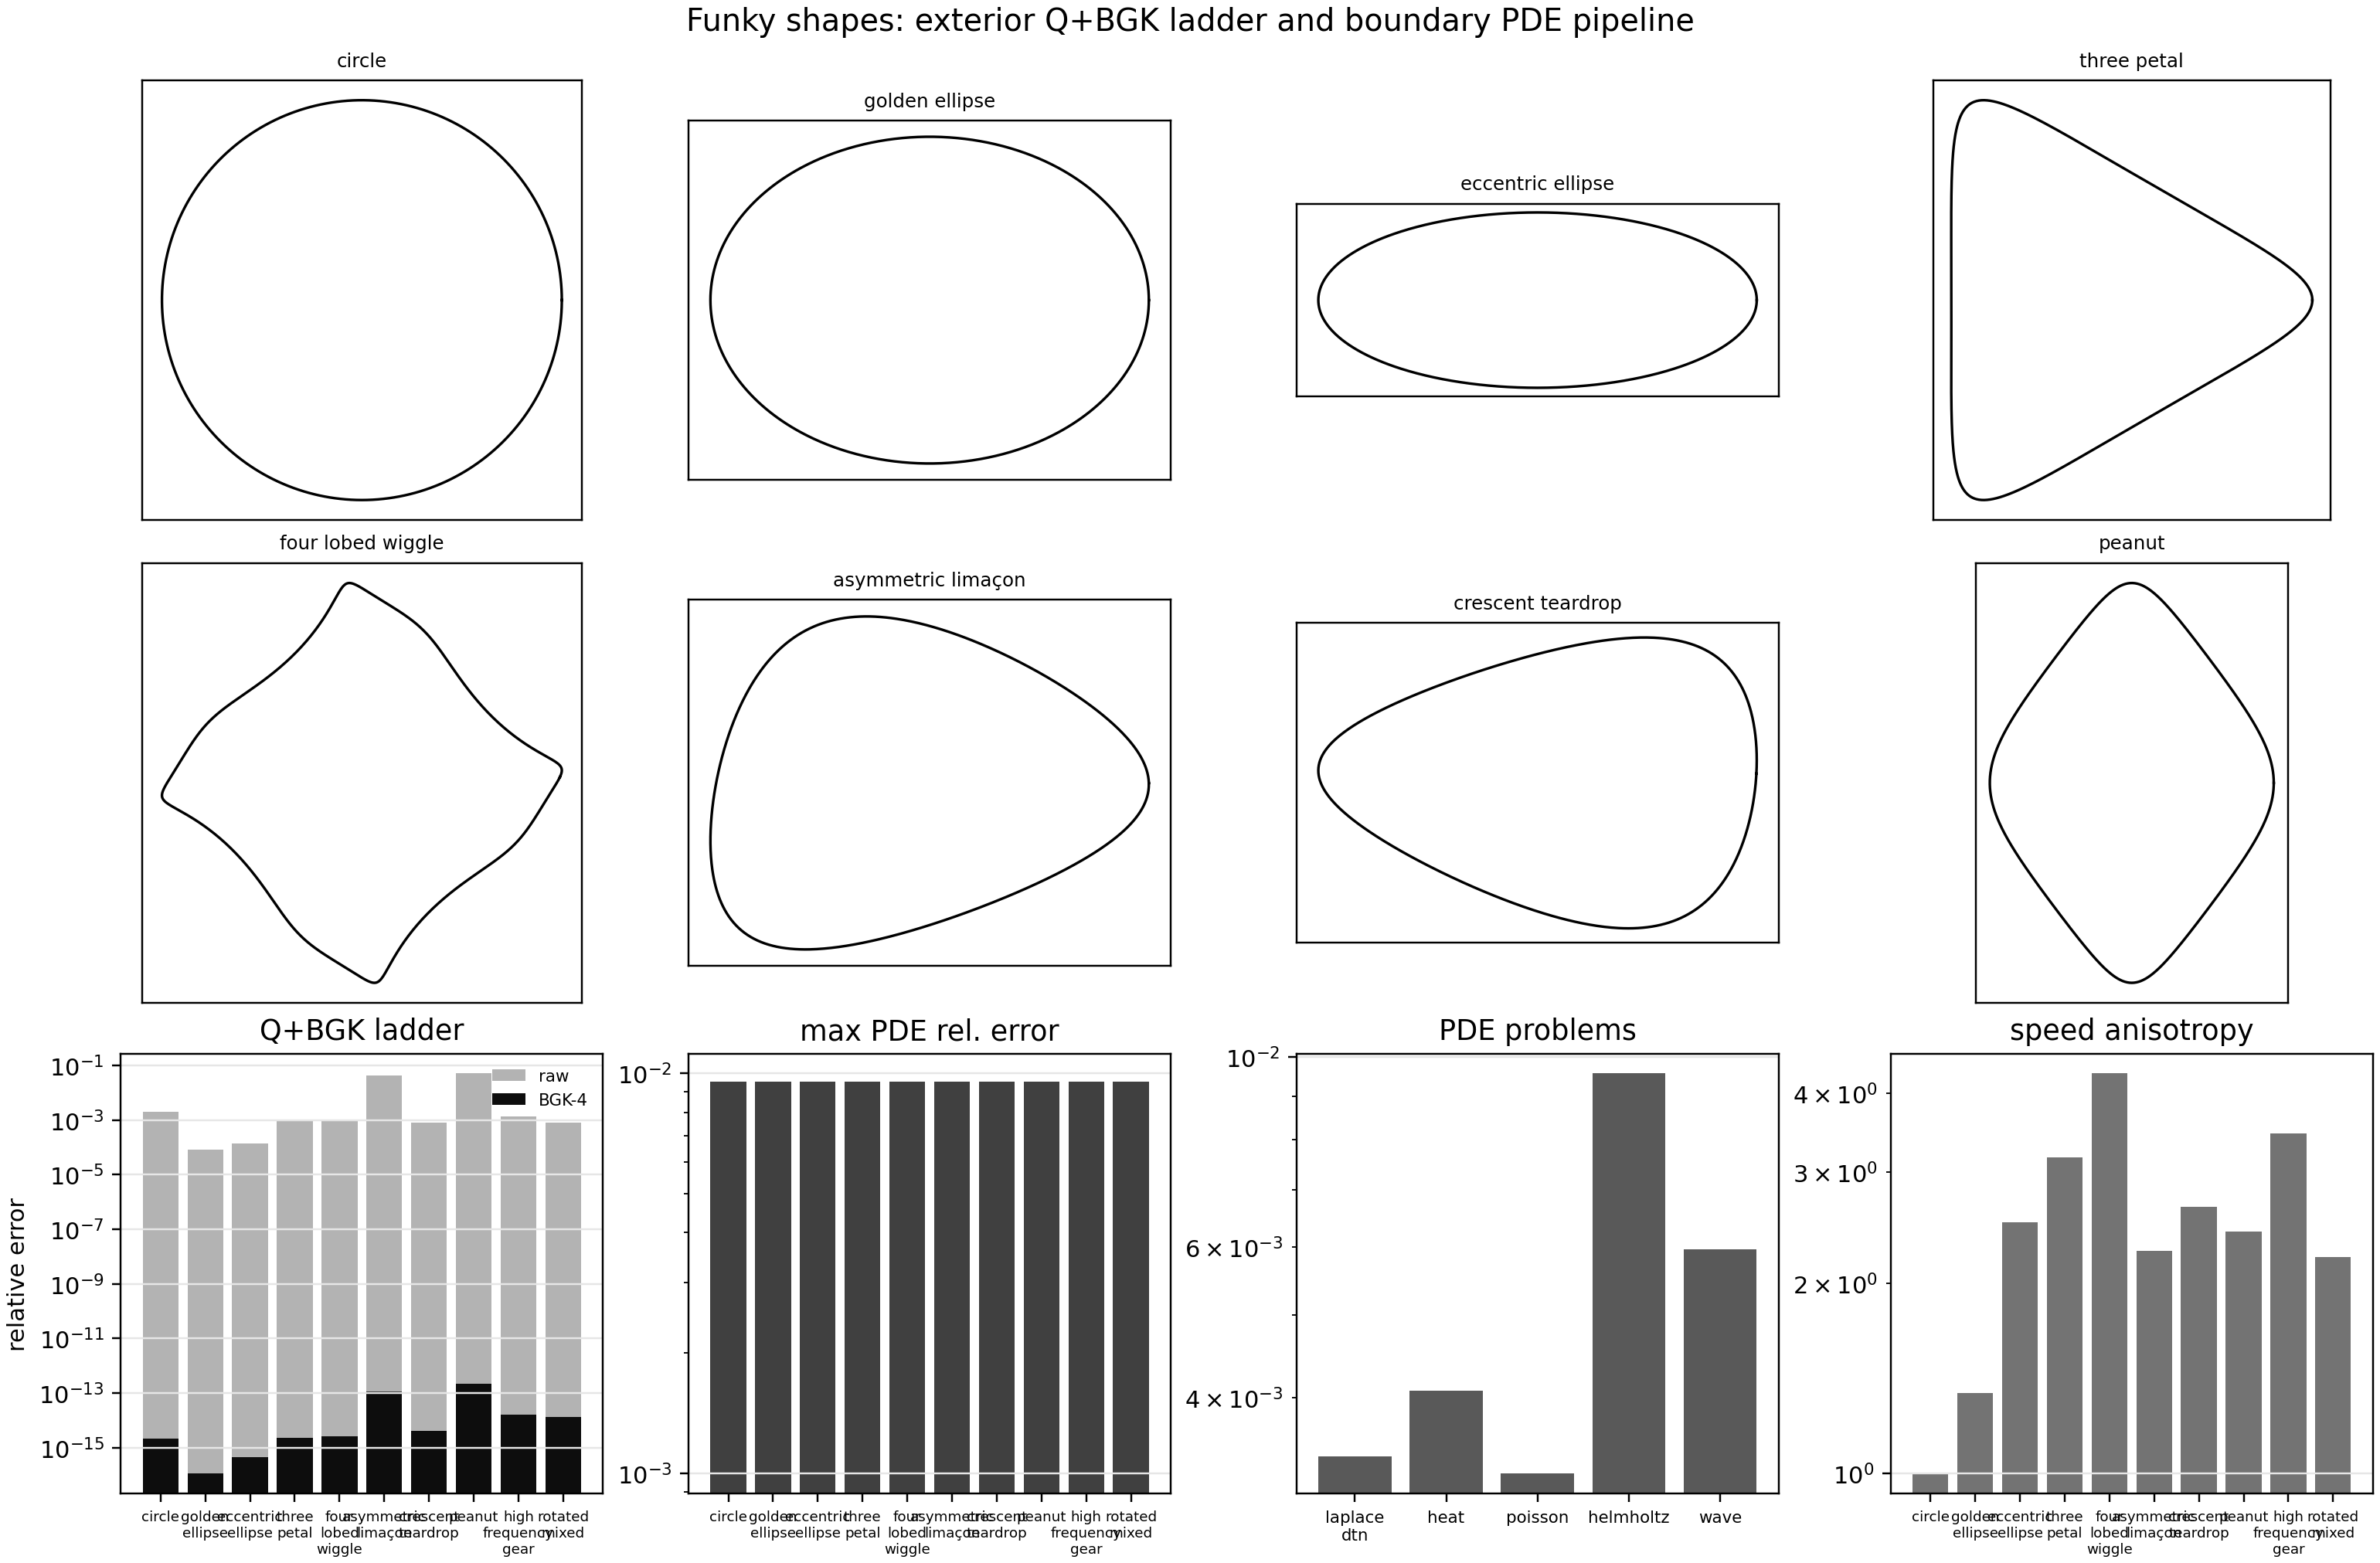
\includegraphics[width=0.92\linewidth]{figures/funky_pde.png}
\caption{Ten exact-Laurent shapes used for Q+BGK quadrature and boundary-only PDE tests.}
\end{figure}
\subsection{Measured matrix-free scaling}
\par\noindent\resizebox{\linewidth}{!}{%
\begin{tabular}{lrrrrr}
\toprule
operation & fit power & ms n=256 & ms n=1024 & ms n=4096 & max residual \\
\midrule
q\_bgk4 & 0.997 & 1.842 & 7.310 & 29.396 & 4.030e-09 \\
pde\_laplace\_dtn & 1.027 & 0.484 & 1.905 & 8.238 & 3.620e-12 \\
pde\_heat & 1.047 & 0.449 & 1.867 & 8.152 & 5.955e-14 \\
pde\_helmholtz & 1.050 & 0.445 & 1.857 & 8.142 & 5.950e-14 \\
pde\_batch\_all5 & 1.047 & 2.262 & 9.353 & 40.943 & 3.620e-12 \\
\bottomrule
\end{tabular}
}\par
\begin{figure}[H]\centering
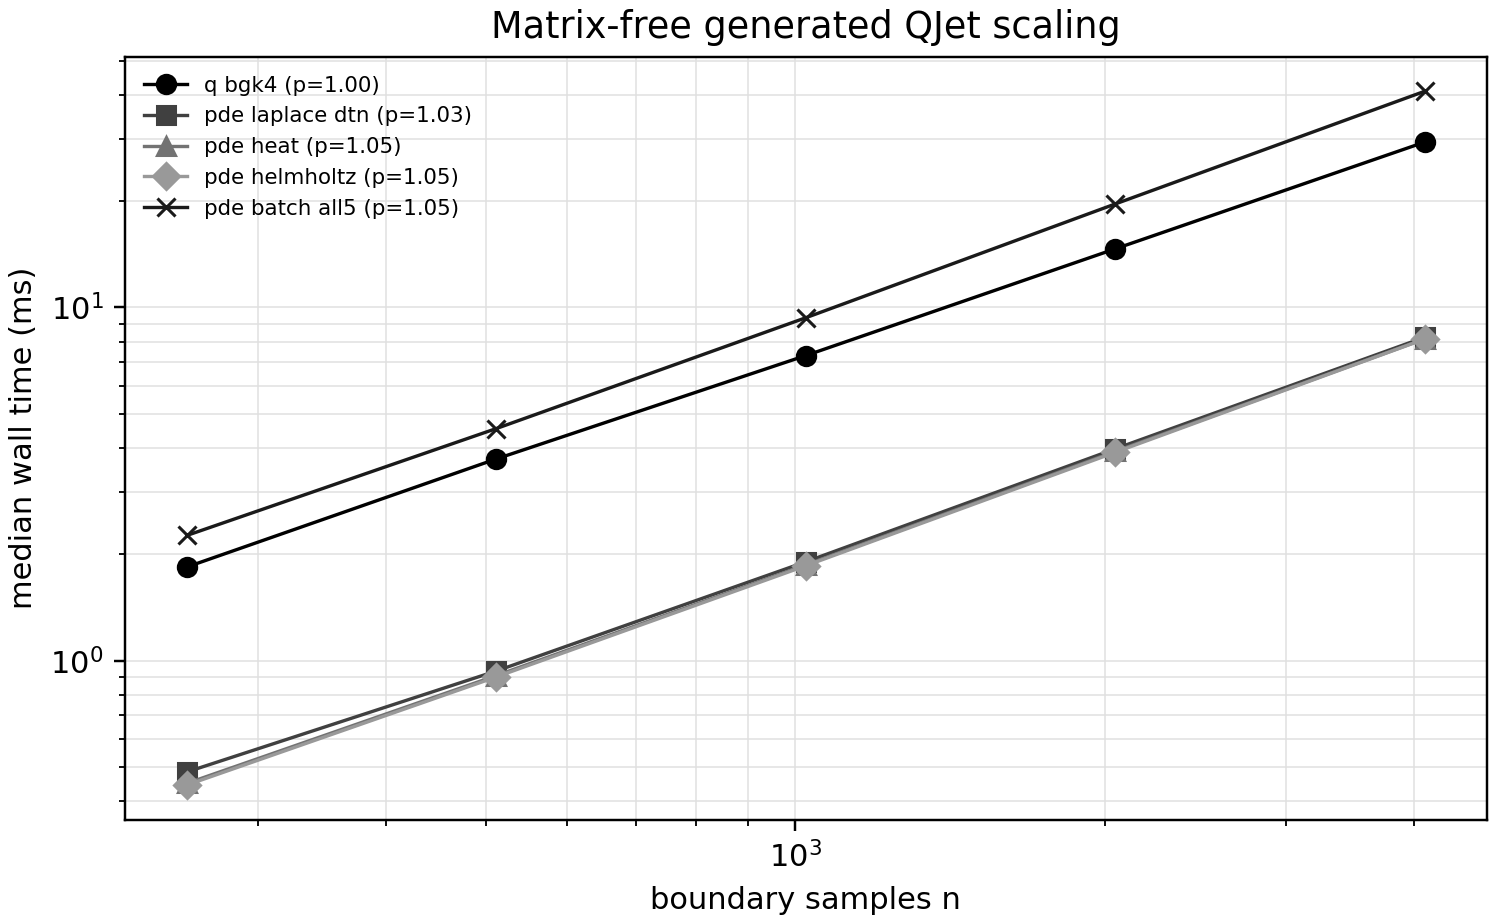
\includegraphics[width=0.78\linewidth]{figures/scaling.png}
\caption{Measured matrix-free scaling.  The fits are near-linear over the tested range and no dense Q matrix is stored.}
\end{figure}
\subsection{Head-to-head methods and Helmholtz caveat}
\par\noindent\resizebox{\linewidth}{!}{%
\begin{tabular}{lrrrrr}
\toprule
method & median err & median ms & work & failures & improvement \\
\midrule
adaptive\_panel & 2.961e-04 & 1.098 & 926.000 & 0 & 36.940 \\
gulati\_q\_bridge & 4.534e-04 & 0.890 & 513.000 & 0 & 12.823 \\
multipole\_zeta\_q & 1.435e-06 & 18.445 & 6.662e+04 & 0 & 5073.817 \\
qbx\_refined & 9.068e-05 & 27.641 & 2.458e+05 & 3 & 159.589 \\
singularity\_subtraction & 4.998e-04 & 0.916 & 533.000 & 0 & 11.182 \\
trapezoid & 0.011 & 0.628 & 512.000 & 0 & 1.000 \\
\bottomrule
\end{tabular}
}\par
\par\noindent\resizebox{\linewidth}{!}{%
\begin{tabular}{ll}
\toprule
suite & result \\
\midrule
disk modal exact & 14 Q wins / 1 FEM wins \\
manufactured exact & 39 Q wins / 1 FEM wins \\
median Q manufactured error & 2.077e-08 \\
median FEM manufactured error & 0.175 \\
\bottomrule
\end{tabular}
}\par
\begin{figure}[H]\centering
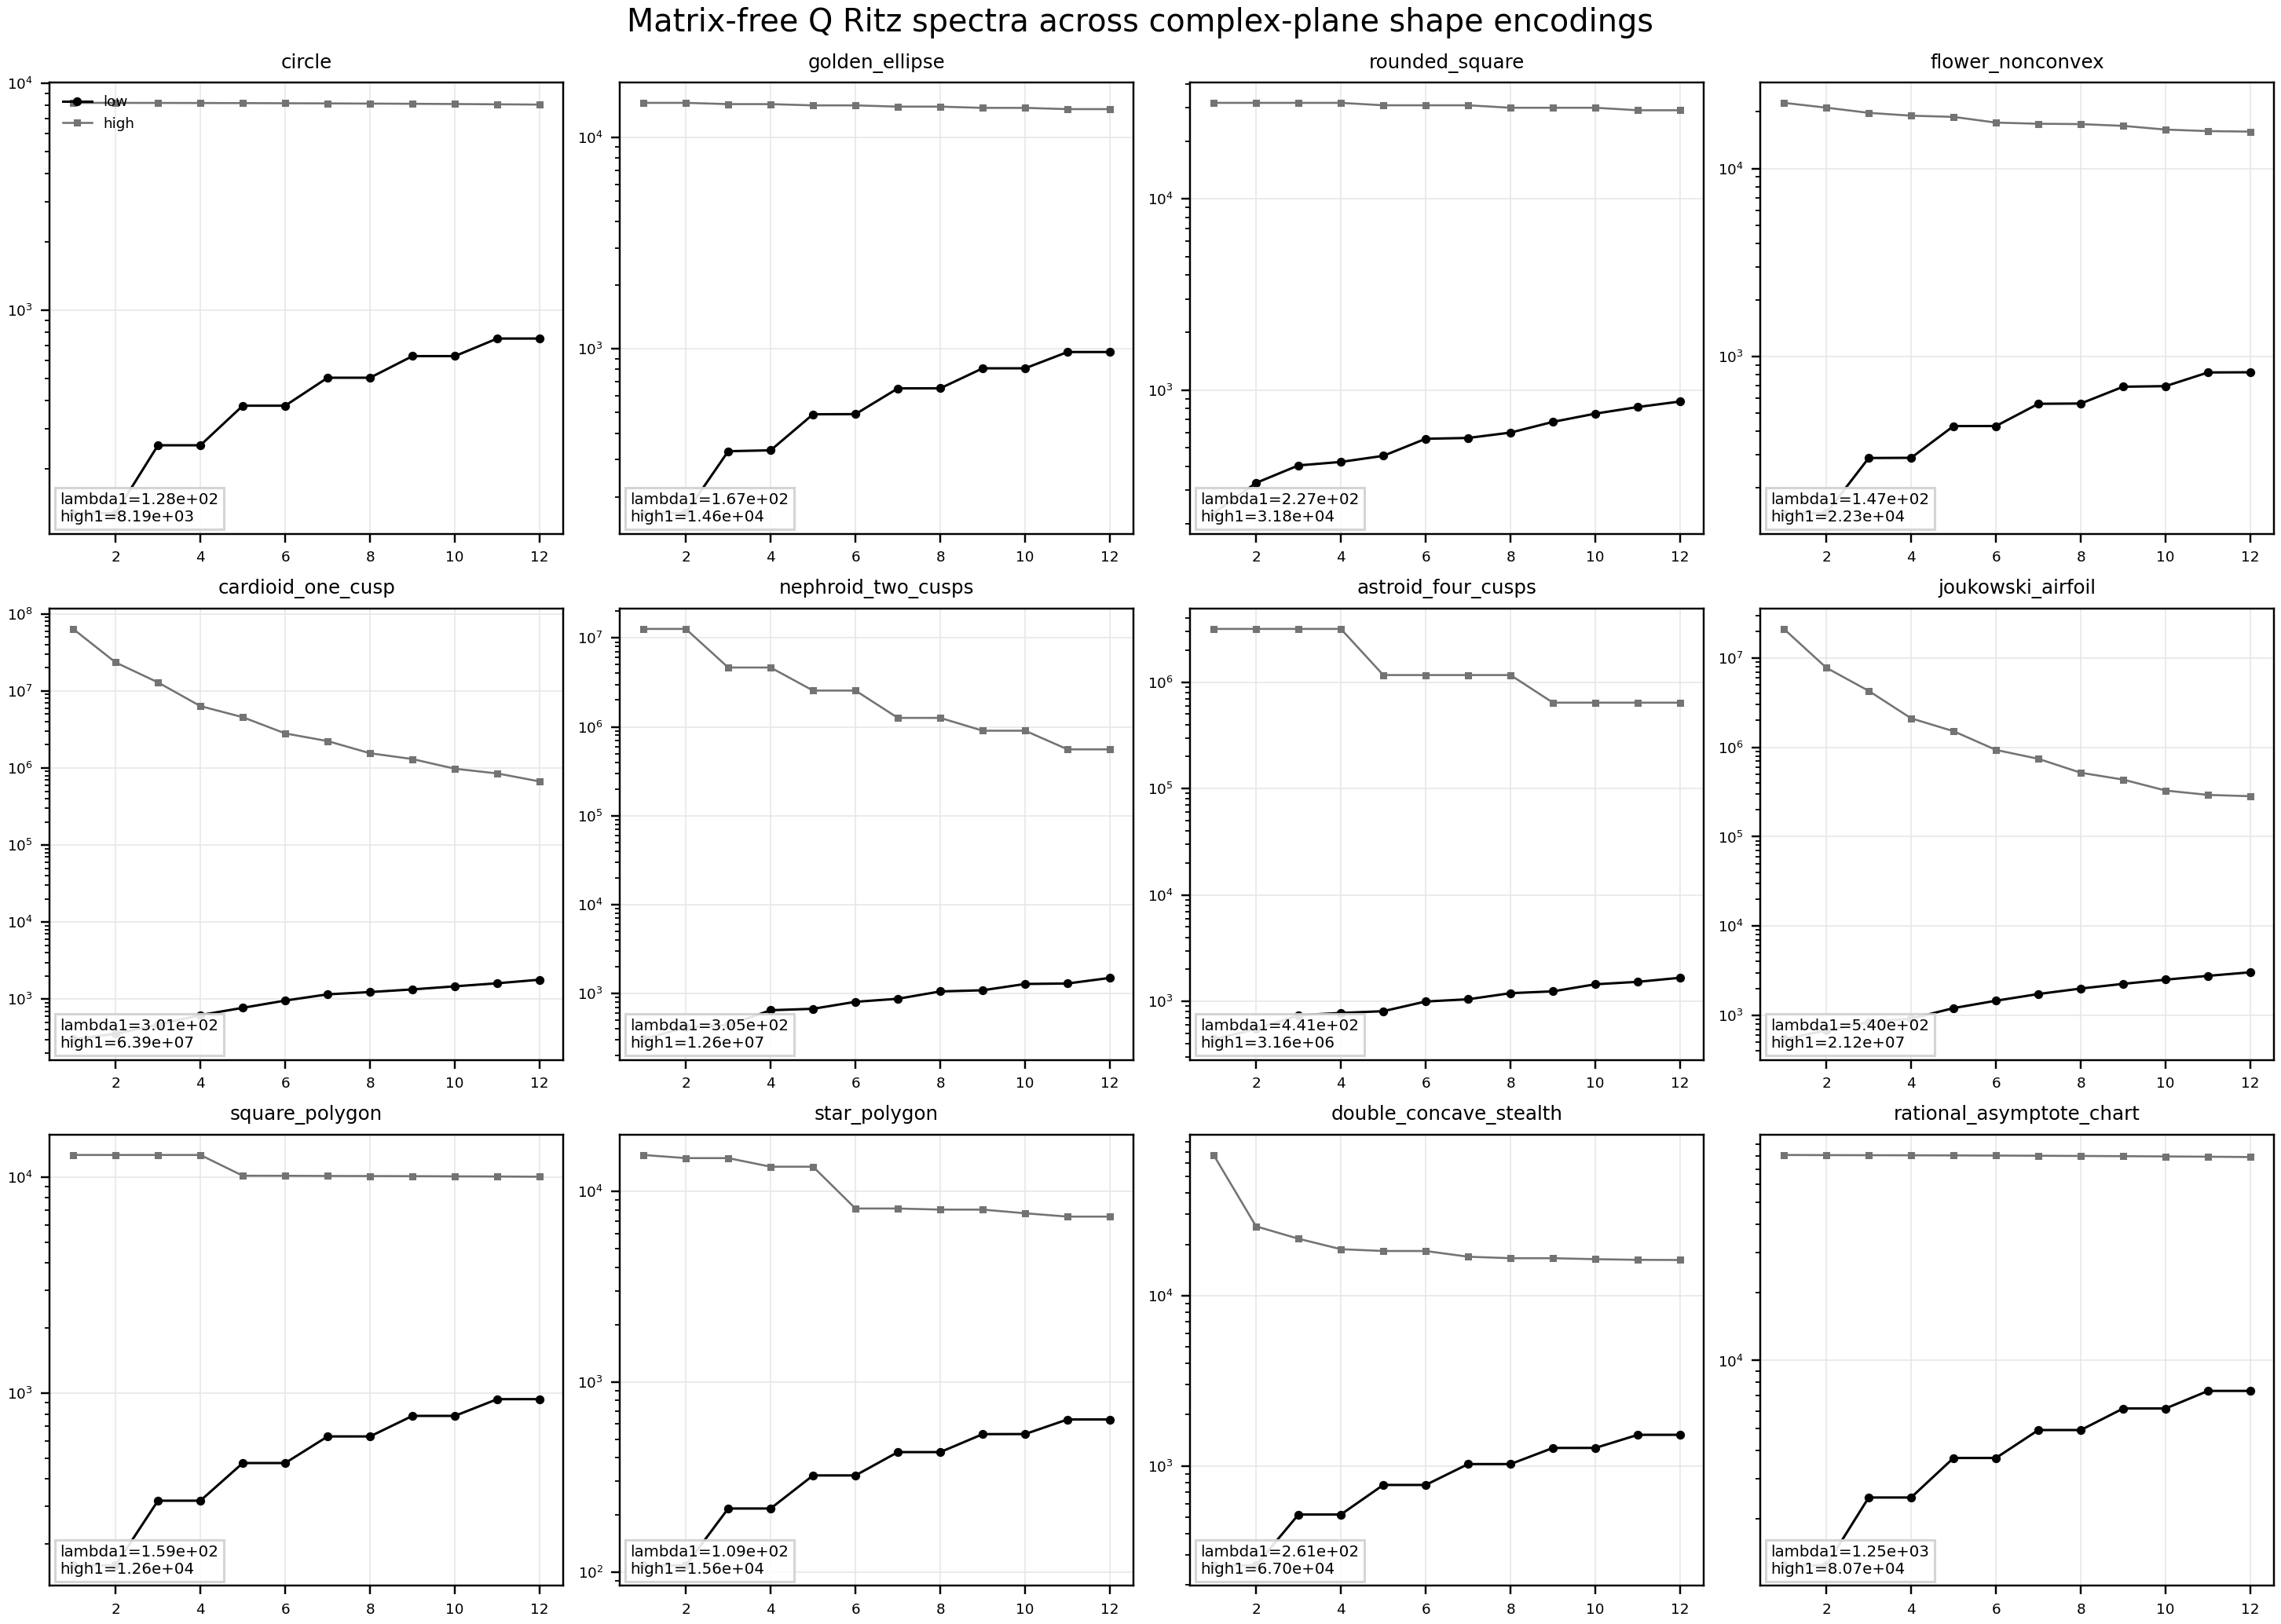
\includegraphics[width=0.92\linewidth]{figures/spectrum.png}
\caption{Q spectrum gallery.  The spectrum diagnoses whether the active error channel is smooth-tail, corner, cusp, or mixed.}
\end{figure}
\begin{figure}[H]\centering
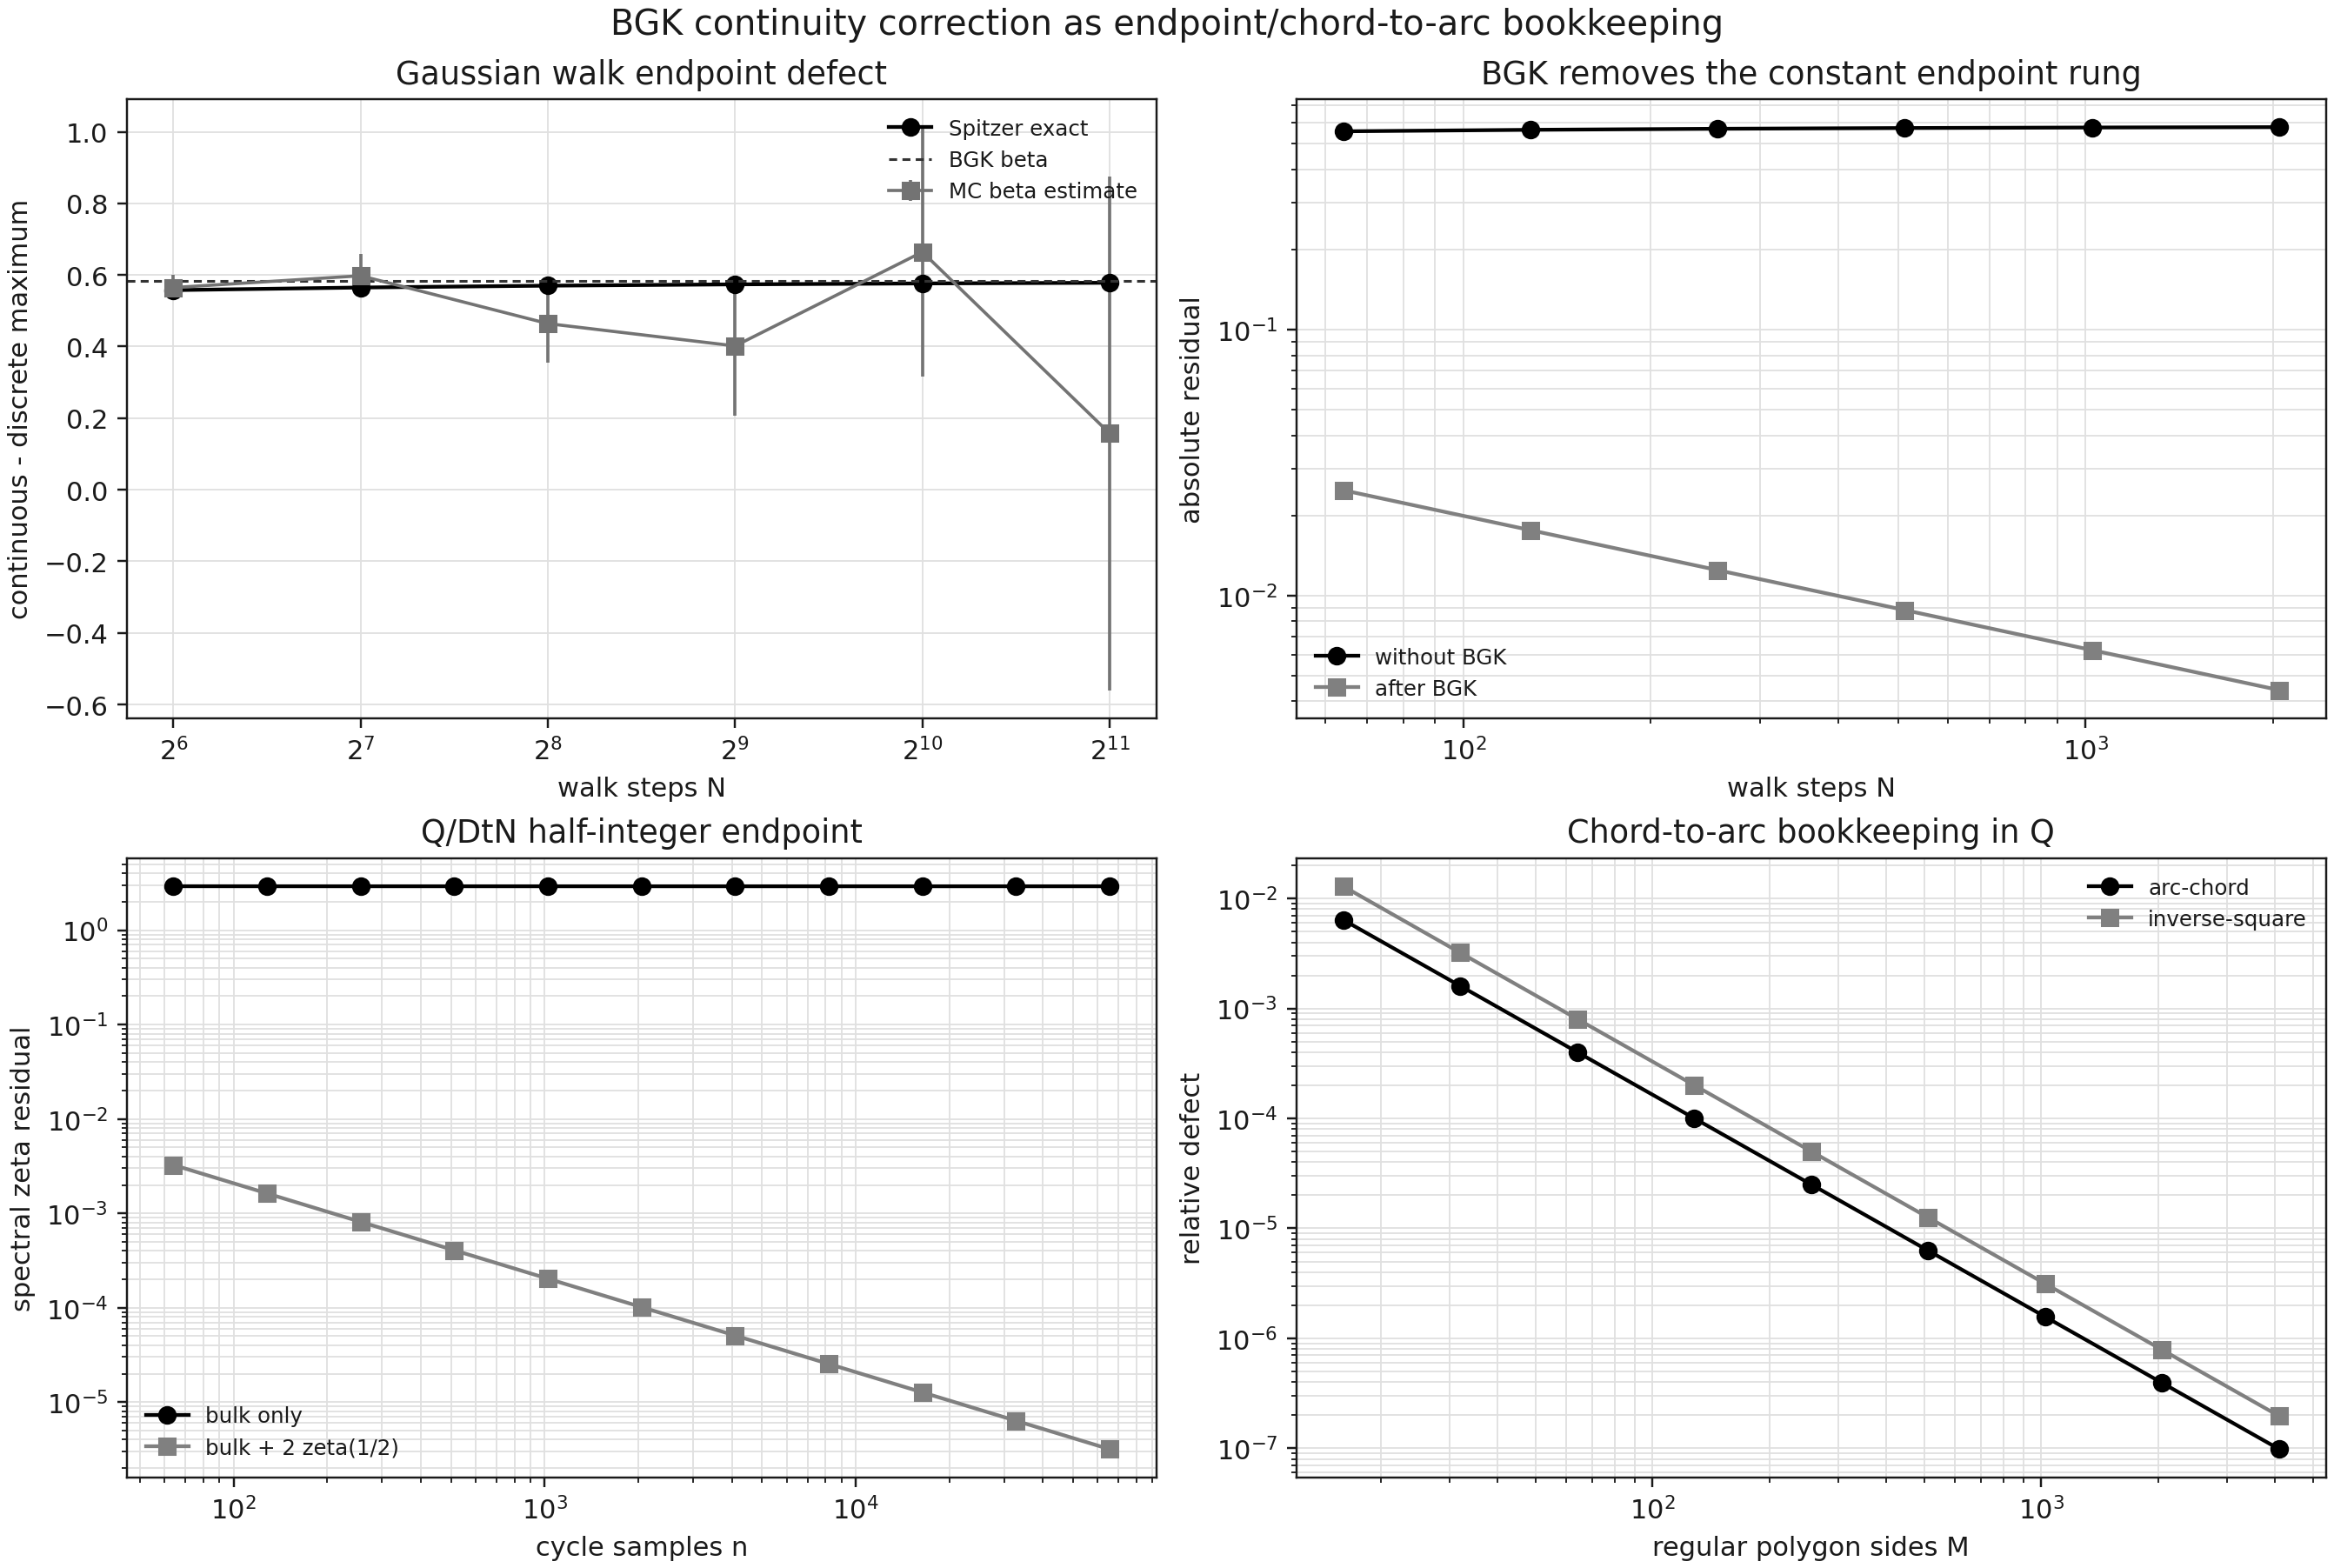
\includegraphics[width=0.88\linewidth]{figures/bgk_bookkeeping.png}
\caption{BGK endpoint bookkeeping as Spitzer, zeta, and Q/DtN endpoint defect.}
\end{figure}
\section{Implementation Contract}
The production implementation follows three invariants.
\begin{enumerate}
\item Store QJets, spectra, Laurent coefficients, samples, and low-rank correction modes; do not store a dense Q matrix.
\item Use the custom QJet Fourier kernel for the singular term and repay geometry through analytic quotients, metric factors, or endpoint/corner ledgers.
\item Report both continuum error and generated-Q residual.  The latter verifies the implementation; the former measures finite-$n$ approximation to the limiting operator.
\end{enumerate}

\subsection{Final self-contained artifact}
The repository contains a final script and a companion notebook generated from the same source.  The script uses no NumPy, no SciPy, and no imported FFT package; its radix-two QJet FFT is implemented directly.  Python library calls are used only for ordinary scalar math, timing, and file output.  The notebook embeds the full script source in a code cell rather than delegating to an external module, so the executable numerical path is auditable from a single \texttt{.ipynb} file.
\par\noindent\resizebox{\linewidth}{!}{%
\begin{tabular}{ll}
\toprule
quantity & value \\
\midrule
pass gate & true \\
machine tolerance & 1.000e-12 \\
max split rel. error & 5.094e-14 \\
max BGK-8 rel. error & 2.231e-13 \\
max generated-Q PDE residual & 6.385e-13 \\
shape count & 10 \\
PDE case count & 50 \\
dense Q matrix stored & false \\
FFT kernel & custom radix-two QJet FFT \\
script & scripts/final\_q\_machine\_precision\_pipeline.py \\
notebook & notebooks/q\_machine\_precision\_pipeline.ipynb \\
\bottomrule
\end{tabular}
}\par
The gate in this table is deliberately stricter than the qualitative plots: the final script fails if the maximum of the split quadrature error, the order-eight BGK repayment error, and the generated-Q PDE residual exceeds $10^{-12}$ over the included finite-Laurent shape suite.

\section{Source Audit}
The following local PDFs were inspected mechanically with \texttt{pdfinfo} and \texttt{pdftotext}.  The audit is not a bibliography; it records which local source artifacts were available while drafting the paper.
\par\noindent\resizebox{\linewidth}{!}{%
\begin{tabular}{lrrrl}
\toprule
PDF & pages & sha & words & role \\
\midrule
optimal\_quad\_merged (26).pdf & 30 & bf3136b87fff & 23511 & early optimal-Q source; benchmark claim cross-check \\
optimal\_quad\_merged (37).pdf & 36 & 858c2f2c1307 & 27573 & later merged optimal-Q source; benchmark claim cross-check \\
optimal\_q\_v63\_public (11).pdf & 20 & 4abcea7d81a5 & 9950 & kernel split, circle pullback, QBX/corner claim boundary \\
isl\_hessian\_v5 (6) copy.pdf & 125 & 629ba599ec42 & 35635 & ellipse/Hessian/context audit; not a numerical benchmark source \\
paper.pdf & 16 & d21c39942f54 & 5377 & meshless shape-optimization/autograd context audit \\
cauchy\_transport\_trim (13).pdf & 18 & bb886ba4ecf6 & 13646 & Cauchy transport early source; pullback notation audit \\
cauchy\_transport\_trim (41).pdf & 25 & c94caccfd128 & 18029 & corner/Joukowski/Kondratiev source audit \\
cauchy\_transport\_trim (47).pdf & 27 & 238918055f3b & 19298 & complex scale-phase pullback source audit \\
cauchy\_transport\_trim (49).pdf & 27 & 131d02d62832 & 19295 & ellipse/de Moivre correction source audit \\
cauchy\_transport\_trim (73).pdf & 29 & c0c8e5932760 & 21896 & latest complex pullback and de Moivre source audit \\
golden\_branch\_outline.pdf & 28 & 15d9ae76cea1 & 8317 & golden ellipse/narrative source audit; not a benchmark source \\
dtn\_bgk\_merge (9).pdf & 22 & 26c17a4cbfb2 & 14386 & DtN/BGK/zeta endpoint correction source \\
harmonic\_sp (41).pdf & 31 & 0e3e2bd04390 & 20933 & harmonic sampling and DtN spectrum source \\
geometry\_of\_money (16).pdf & 31 & 572cc37c67b0 & 13140 & BGK continuity correction and chord-arc bookkeeping source \\
\bottomrule
\end{tabular}
}\par
\section{Conclusion}
The elegant core is the chain
\[
\frac{1-\cos(2\pi md/n)}{4\sin^2(\pi d/n)}
\longrightarrow
\lambda_{m,n}=\frac{m(n-m)}{2}
\longrightarrow
\mu_{m,n}=m\left(1-\frac mn\right)
\longrightarrow
\Lam_{S^1}=|D|.
\]
This identity supplies the generated Q spectrum.  The exterior map supplies the split
\[
\log|\psi(w)-\psi(z)|=\log|w-z|+\log|G(w,z)|,
\]
and the endpoint calculus supplies the BGK/zeta repayment
\[
\beta=-\zeta(1/2)/\sqrt{2\pi}.
\]
Together these identities explain why the exact analytic path reaches machine precision, why the PDE pipeline can use Q as an operator rather than a post-process, and why the spectrum is the correct diagnostic for deciding whether smooth, corner, cusp, or Helmholtz-specific corrections are required.

\begin{thebibliography}{9}
\bibitem{BGK}
M. Broadie, P. Glasserman, and S. Kou, A continuity correction for discrete barrier options, \emph{Mathematical Finance}, 7 (1997), pp. 325--349.
\bibitem{GWW}
C. Gordon, D. Webb, and S. Wolpert, One cannot hear the shape of a drum, \emph{Bull. Amer. Math. Soc.}, 27 (1992), pp. 134--138.
\bibitem{QBX}
A. Klockner, A. Barnett, L. Greengard, and M. O'Neil, Quadrature by expansion: A new method for the evaluation of layer potentials, \emph{J. Comput. Phys.}, 252 (2013), pp. 332--349.
\bibitem{Spitzer}
F. Spitzer, A combinatorial lemma and its application to probability theory, \emph{Trans. Amer. Math. Soc.}, 82 (1956), pp. 323--339.
\bibitem{TW}
L. N. Trefethen and J. A. C. Weideman, The exponentially convergent trapezoidal rule, \emph{SIAM Review}, 56 (2014), pp. 385--458.
\end{thebibliography}
\end{document}
